\chapter{Results}
\label{ch:ch4}
In this chapter, we present the results of the normal mode decomposition compared to the Helmholtz decomposition. In addition to examining the decomposition as a function of vertical mode number, we focus attention on the mesoscale. The discussion and analysis of these results is saved until Chapter \ref{ch:ch5}.

\section{Normal Mode Decomposition}
\subsection{Individual Vertical Modes}
The normal mode decomposition described in Chapter \ref{ch:ch2} is different than the Helmholtz decomposition for a few reasons. The normal mode decomposition splits the total energy (kinetic plus potential) into geostrophic and ageostrophic motion. The normal mode decomposition also provides a way to look at the energy contained in each vertical mode and how the geostrophic and ageostrophic spectra vary as the vertical scale gets smaller.\\

Applying the normal mode decomposition to the jet described in Chapter \ref{ch:ch3} leads to the normal mode structure seen in Figure \ref{fig:normalmodes}, as well as equivalent depths in Table \ref{tab:equivDepths}. Once the normal modes are solved, we project the horizontal velocity and geopotential fields to each mode. First, we show the barotropic mode in Figure \ref{fig:barotropicKEPE}, which corresponds to vertical mode 0. The largest scales corresponding to the smallest non-dimensional wavenumbers, $\tilde{k} = L_x/2\pi |\mathbf{k}|$, represent wavelengths of around 5000 km, while the largest values of $\tilde{k}$ represent wavelengths as small as 10 km. The mesoscale is shown around $\tilde{k} \approx 6$ to 60. Near the larger wavenumbers, at  $\tilde{k} \approx 300$, the spectra quickly steepen as the energy contained at these scales goes to zero. This is due to the numerical dissipation inherent in the WRF discretization. Finally, since the energy is binned over circles of constant radius in the $k-l$ plane according to equation (\ref{eq:binning}), all of the energy that is outside the circle of radius $\tilde{k}_{\text{max}} = 512$ is binned together at the end.\\

The barotropic mode is qualitatively a little different from the baroclinic modes. Perhaps the most notable difference of the barotropic mode is the difference between the DKE and ageostrophic spectra. The DKE of the barotropic mode is very different from the ageostrophic mode, where the ageostrophic spectrum stays roughly constant at a -4.0 slope across all length scales, while  DKE spectrum rapidly shallows from a -3.7 slope in the synoptic scale to a -2.6 slope in the mesoscale. The vertical structure of the barotropic mode is nearly constant, which corresponds to the largest equivalent depth.  \\

Each vertical mode from the normal mode decomposition employed in this thesis is a boundary value problem that covers the full extent of the atmosphere. For this reason, to best make a comparison to the Helmholtz decomposition, we average the 2D horizontal RKE and DKE spectra over the entire depth of the atmosphere. This is different from most of the literature (e.g. \cite{Hamilton2008}, \cite{Skamarock2008a}, \cite{Waite2009}, \cite{Peng2013}, \cite{Waite2013}), which averages over different regions of the atmosphere (e.g. upper troposphere, tropopause, stratosphere), or consider specific vertical levels, due in part to the different stratification profiles. 

\begin{figure}[H]
\vspace{-3cm}
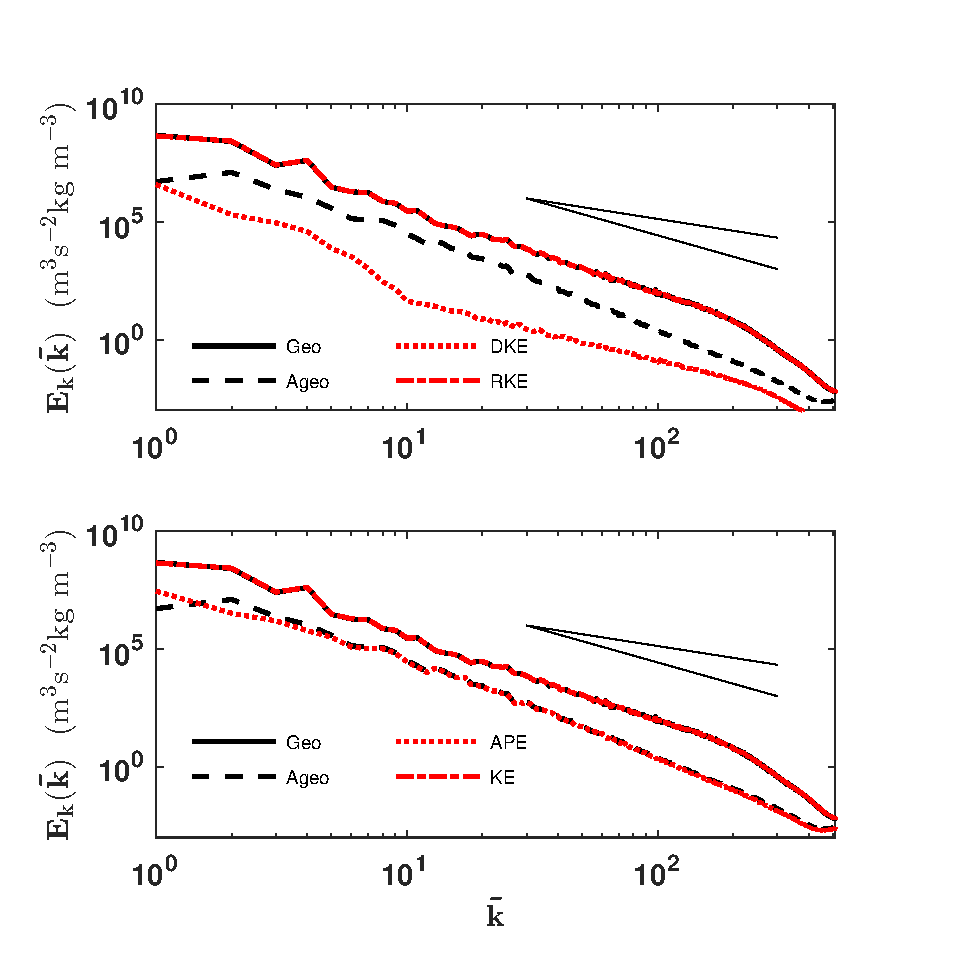
\includegraphics[scale=1]{Chapter4/img/GeoAgeoBarotropic}
\vspace{-1cm}
\caption{Energy spectra of barotropic mode. The top shows the geostrophic (black solid) and ageostrophic (black dashed) modes along with the rotational (red dash-dot) and the divergent (red dotted) kinetic energy spectra. The bottom shows the geostrophic (black solid) and ageostrophic (black dashed) modes versus the kinetic energy (red dash-dot) and potential energy (red dotted). Reference lines with $-5/3$ and $-3$ slopes are shown in the upper right.}
\label{fig:barotropicKEPE}
\end{figure}

The baroclinic modes correspond to normal modes with changing vertical structure. As the mode number increases, the equivalent depth of the associated shallow water system decreases as well as the number of zero crossings, which corresponds to a length scale that can be thought of as a ``wavelength'' of the vertical mode. Figures \ref{fig:GeoAgeo_RKEDKE_1-3} - \ref{fig:GeoAgeo_RKEDKE_29} show the energy spectra of the first 30 baroclinic modes. For conciseness, only the odd numbered vertical modes are shown.\\

In the baroclinic modes, it is immediately apparent that there is closer agreement between the DKE spectrum and the ageostrophic spectrum slopes. For the first several vertical modes, the rotational kinetic energy spectrum and the geostrophic energy spectrum agree well at all but the largest of scales. It is also evident that with increasing vertical mode number, the RKE and DKE spectra begin to shallow at a much more pronounced rate than the geostrophic and ageostrophic spectra (see Figure \ref{fig:slopes}). Another observation from the baroclinic spectra show that as the vertical mode number increases, the energy in the mesoscale increases in the geostrophic and DKE spectra. \\

\begin{figure}[H]
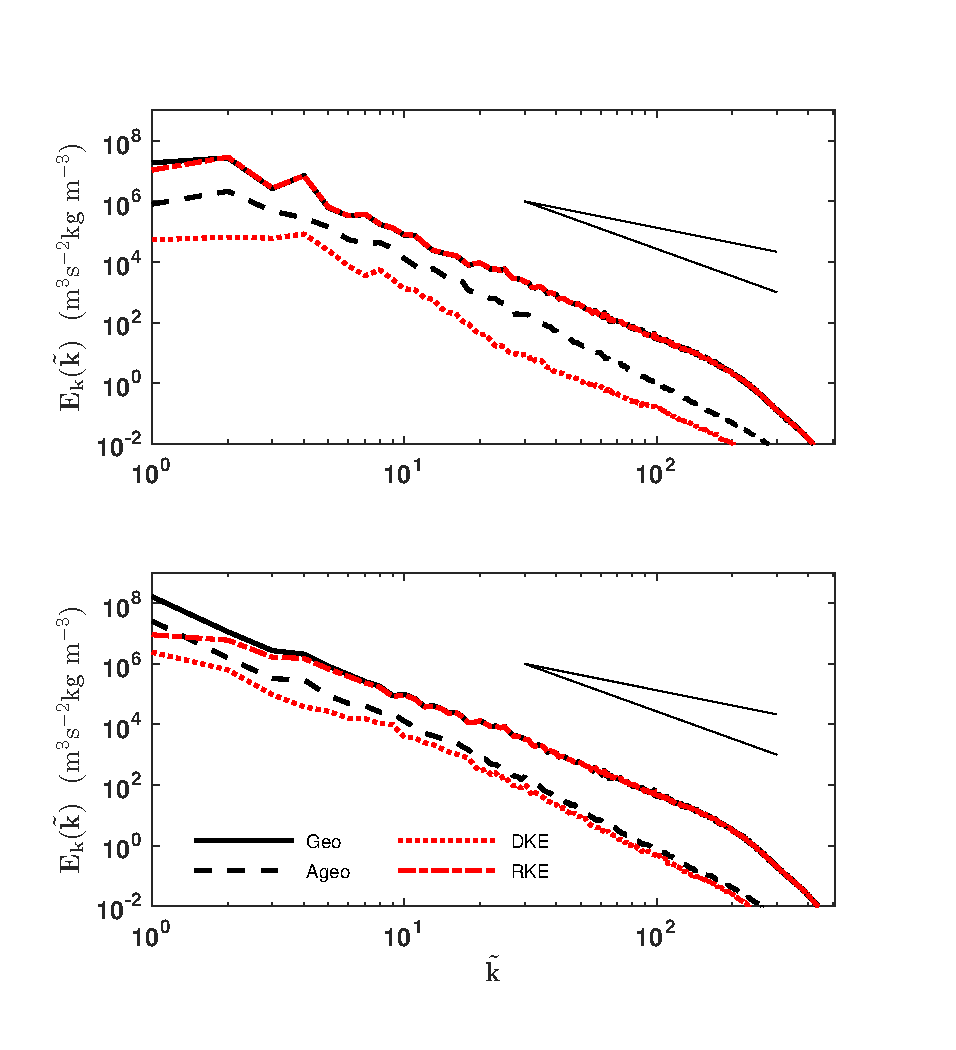
\includegraphics[scale=1]{Chapter4/img/GeoAgeo_RKEDKE_1-3}
\vspace{-3em}
\caption{Vertical modes 1 (top) and 3 (bottom). Both figures show the geostrophic (black solid) and ageostrophic (black dashed) modes compared to the RKE (red dash dot) and DKE (red dotted). $-5/3$ and $-3$ references are shown in the upper right. The wavenumber corresponding to $f/c_n$ is $\tilde{k} = 0.65$ for mode 1 and $\tilde{k} = 1.5$ for mode 3.}
\label{fig:GeoAgeo_RKEDKE_1-3}
\end{figure}

\begin{figure}[H]
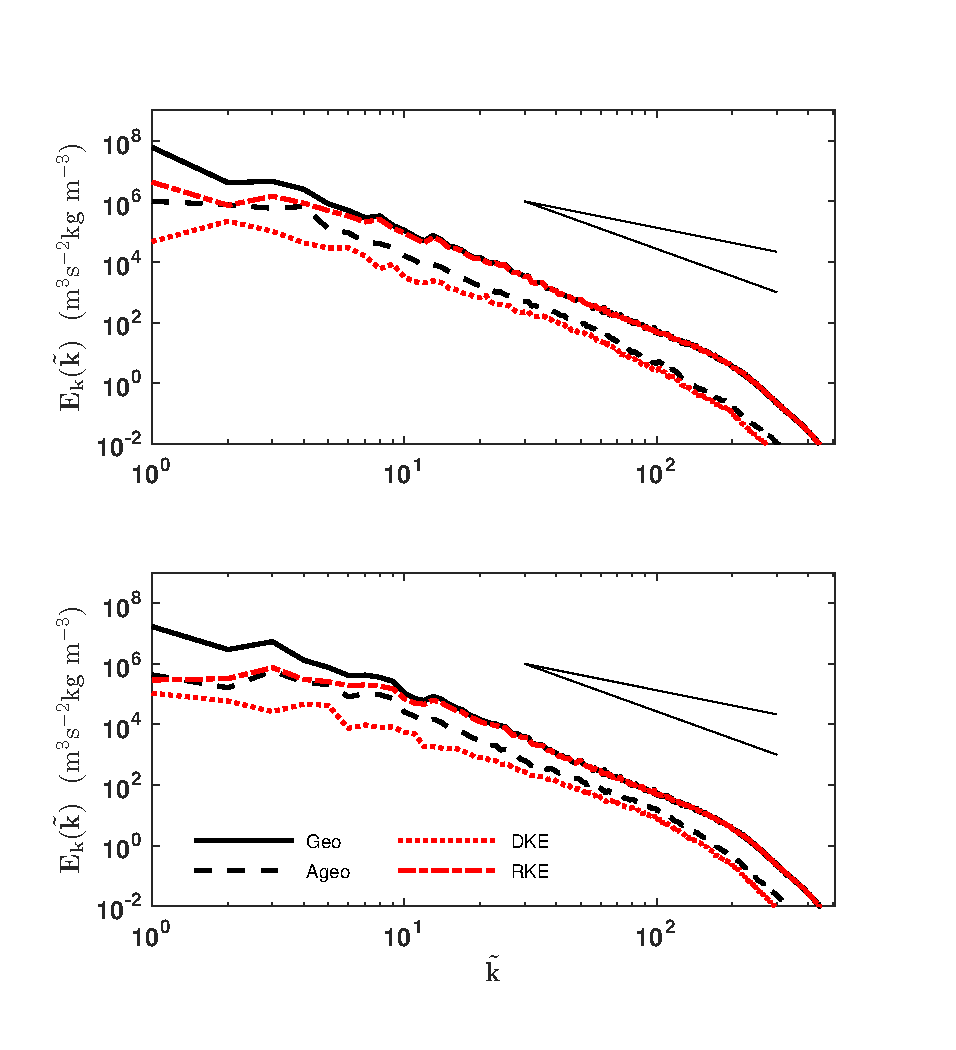
\includegraphics[scale=1]{Chapter4/img/GeoAgeo_RKEDKE_5-7}
\caption{The same as in Figure \ref{fig:GeoAgeo_RKEDKE_1-3}, but for vertical modes 5 (top) and 7 (bottom).  The wavenumber corresponding to $f/c_n$ is  $\tilde{k} = 2.5$ for mode 5 and $\tilde{k} = 3.6$ for mode 7.}
\label{fig:GeoAgeo_RKEDKE_5-7}
\end{figure}

\begin{figure}[H]
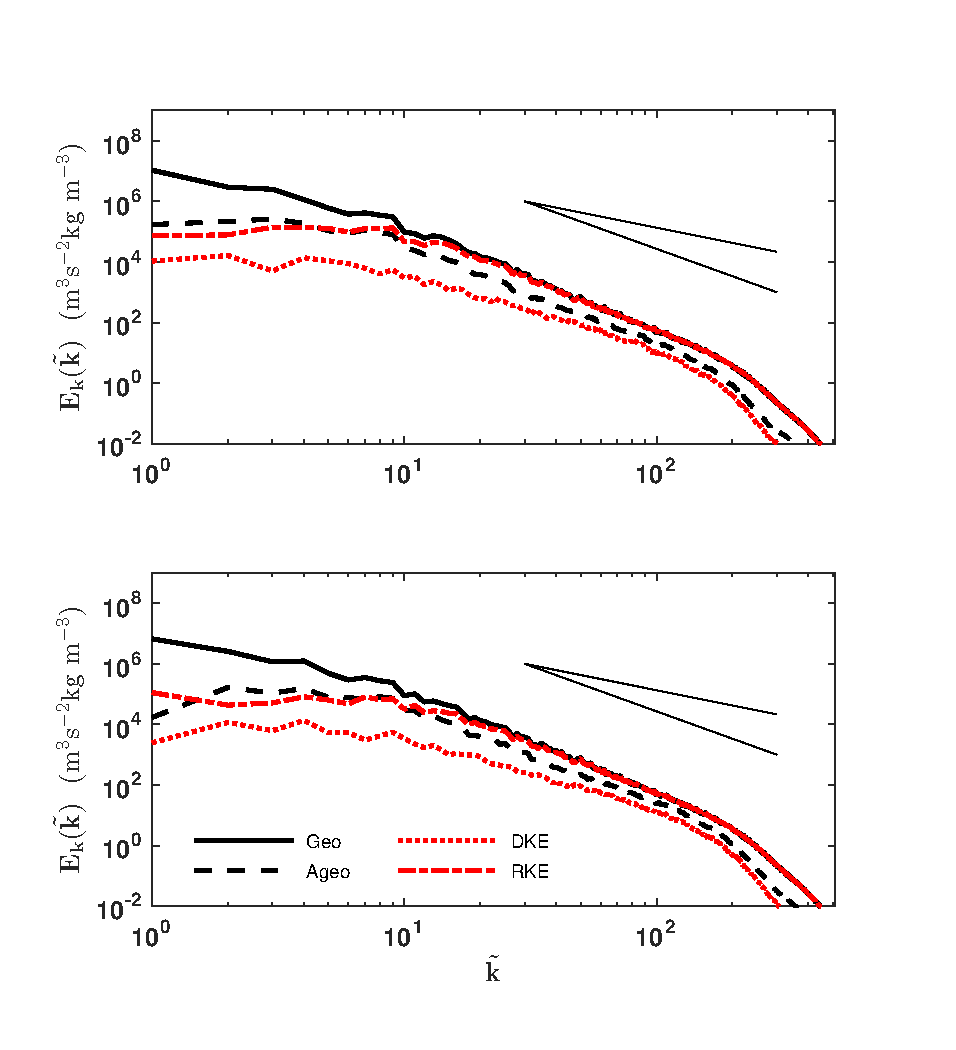
\includegraphics[scale=1]{Chapter4/img/GeoAgeo_RKEDKE_9-11}
\caption{The same as in Figure \ref{fig:GeoAgeo_RKEDKE_1-3}, but for vertical modes 9 (top) and 11 (bottom).  The wavenumber corresponding to $f/c_n$ is $\tilde{k} = 4.9$ for mode 9 and $\tilde{k} = 6.1$ for mode 11.}
\label{fig:GeoAgeo_RKEDKE_9-11}
\end{figure}

\begin{figure}[H]
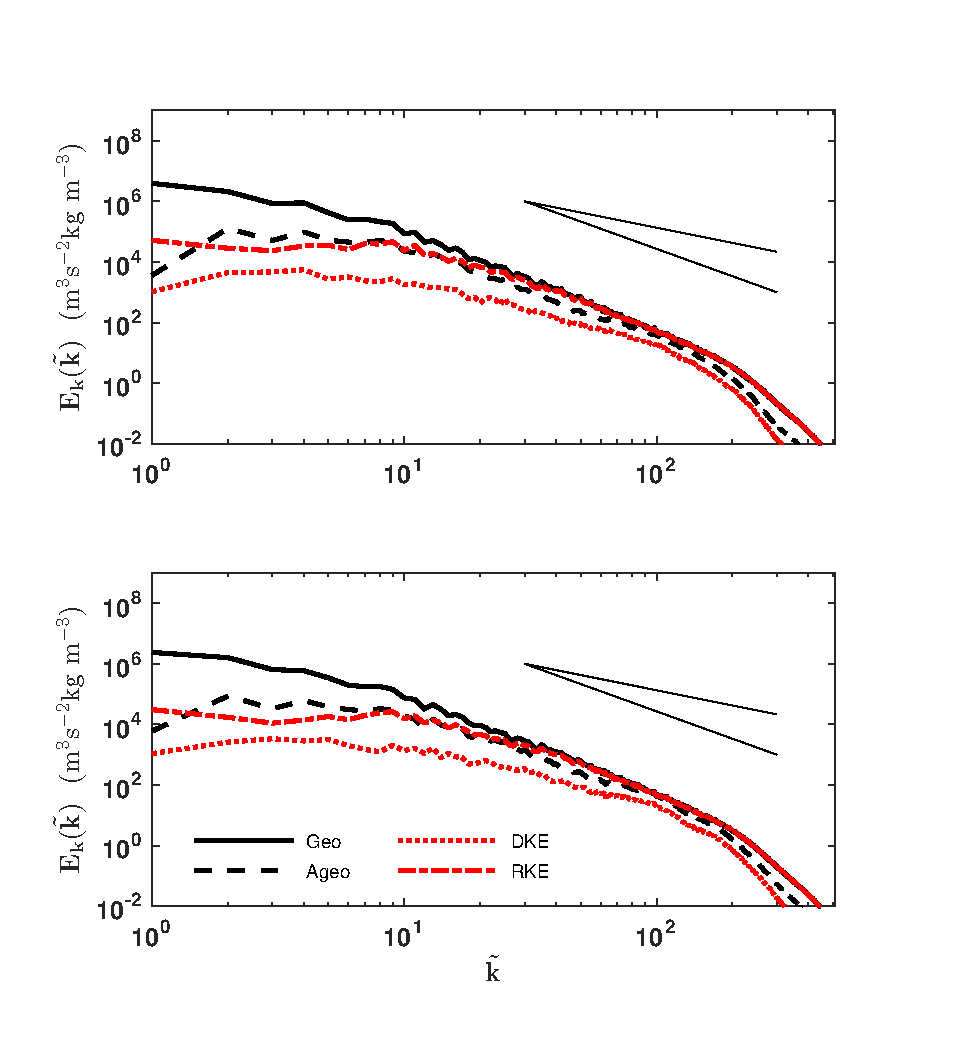
\includegraphics[scale=1]{Chapter4/img/GeoAgeo_RKEDKE_13-15}
\caption{The same as in Figure \ref{fig:GeoAgeo_RKEDKE_1-3}, but for vertical modes 13 (top) and 15 (bottom).  The wavenumber corresponding to $f/c_n$ is $\tilde{k} = 7.5$ for mode 13 and $\tilde{k} = 8.9$ for mode 15.}
\label{fig:GeoAgeo_RKEDKE_13-15}
\end{figure}

\begin{figure}[H]
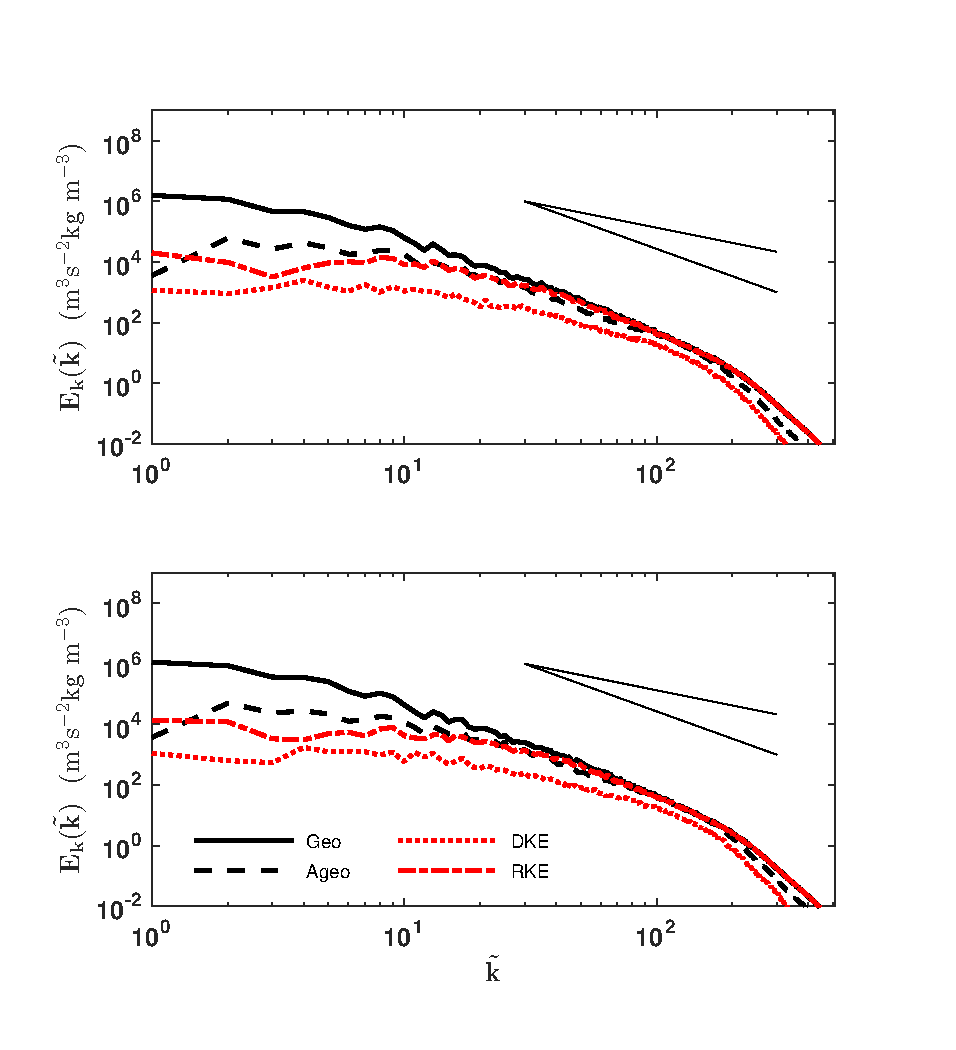
\includegraphics[scale=1]{Chapter4/img/GeoAgeo_RKEDKE_17-19}
\caption{The same as in Figure \ref{fig:GeoAgeo_RKEDKE_1-3}, but for vertical modes 17 (top) and 19 (bottom).  The wavenumber corresponding to $f/c_n$ is $\tilde{k} = 10.3$ for mode 17 and $\tilde{k} = 11.8$ for mode 19.}
\label{fig:GeoAgeo_RKEDKE_17-19}
\end{figure}

\begin{figure}[H]
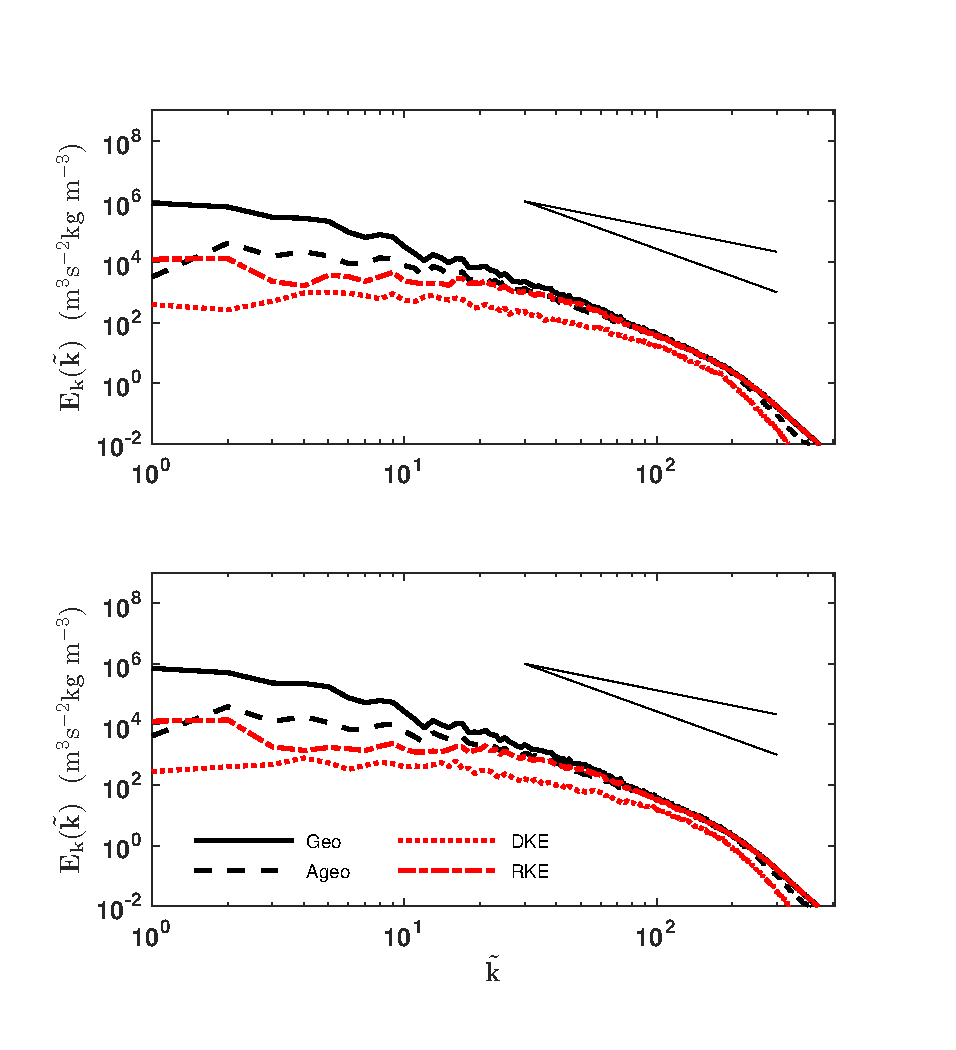
\includegraphics[scale=1]{Chapter4/img/GeoAgeo_RKEDKE_21-23}
\caption{The same as in Figure \ref{fig:GeoAgeo_RKEDKE_1-3}, but for vertical modes 21 (top) and 23 (bottom).  The wavenumber corresponding to $f/c_n$ is $\tilde{k} = 13.4$ for mode 21 and $\tilde{k} = 15$ for mode 23.}
\label{fig:GeoAgeo_RKEDKE_21-23}
\end{figure}

\begin{figure}[H]
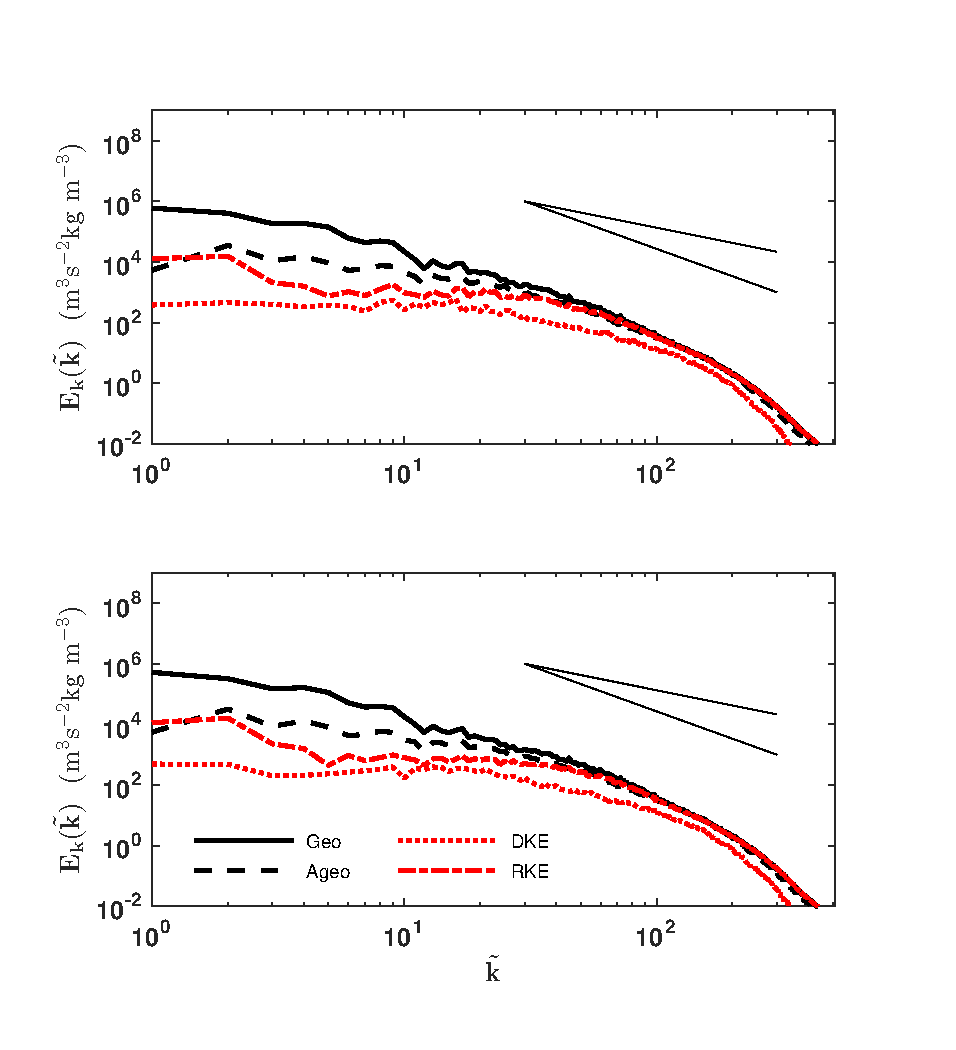
\includegraphics[scale=1]{Chapter4/img/GeoAgeo_RKEDKE_25-27}
\caption{The same as in Figure \ref{fig:GeoAgeo_RKEDKE_1-3}, but for vertical modes 25 (top) and 27 (bottom).  The wavenumber corresponding to $f/c_n$ is $\tilde{k} = 16.6$ for mode 25 and $\tilde{k} = 18.3$ for mode 27.}
\label{fig:GeoAgeo_RKEDKE_25-27}
\end{figure}

\begin{figure}[H]
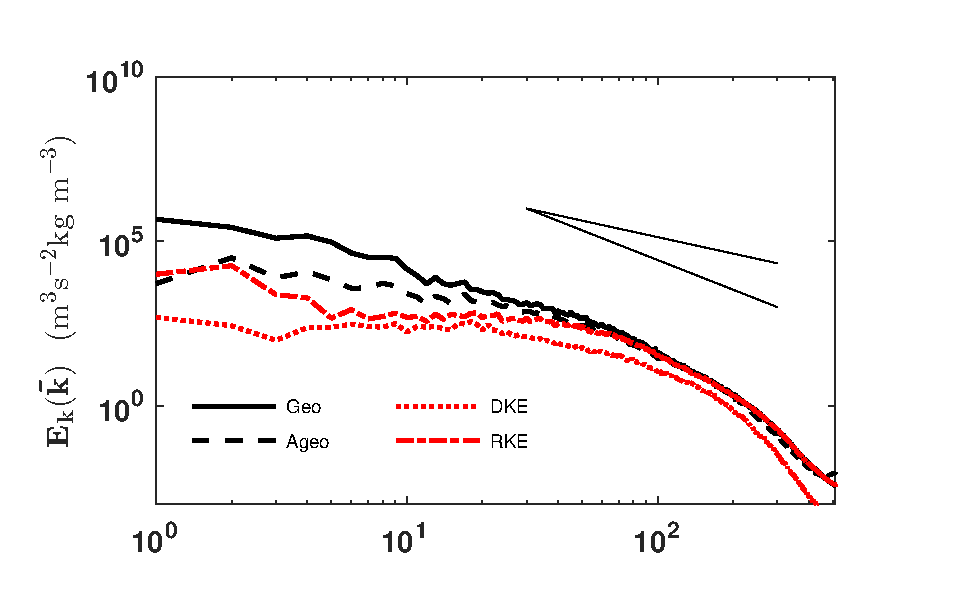
\includegraphics[scale=1]{Chapter4/img/GeoAgeo_RKEDKE_29}
\caption{The same as in Figure \ref{fig:GeoAgeo_RKEDKE_1-3}, but for vertical mode 29.  The wavenumber corresponding to $f/c_n$ for this mode is $\tilde{k} = 20.1$.}
\label{fig:GeoAgeo_RKEDKE_29}
\end{figure}

\subsection{Examining the Composition of the Normal Modes}
It is also useful to compare to include the potential energy alongside the RKE and DKE  to further understand the role each of these quantities have in establishing the geostrophic and ageostrophic spectra. Figures \ref{fig:Geo_APERKE_1-3} - \ref{fig:Geo_APERKE_29} show the geostrophic modes along with the RKE and available potential energy (APE) per vertical mode. Since the geostrophic mode is non-divergent, the DKE is omitted for clarity. Unlike the geostrophic modes, the ageostrophic modes have non-zero divergence. Figures \ref{fig:Ageo_APEDKE_1-3} - \ref{fig:Ageo_APEDKE_29} show the ageostrophic modes with the DKE, RKE, and APE per vertical mode.

%%%%%%%%%%%%
\begin{figure}[H]
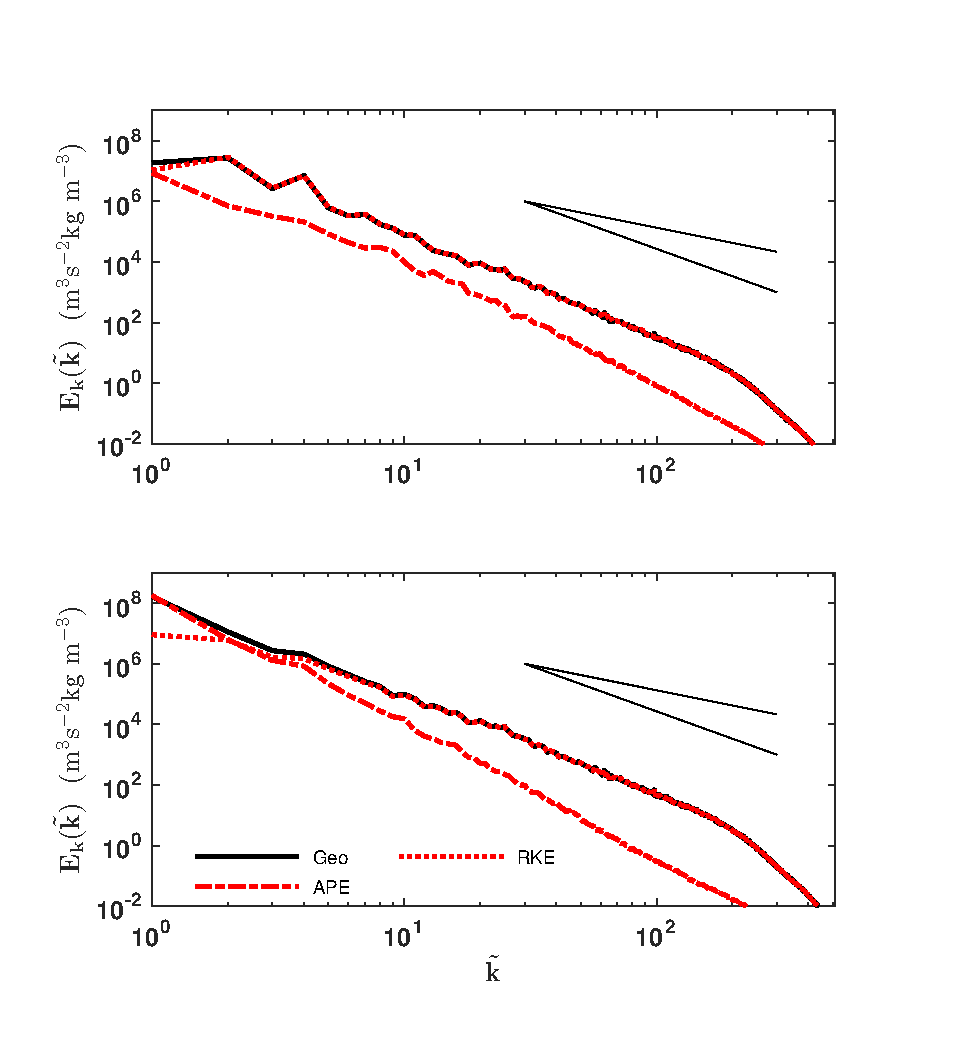
\includegraphics[scale=1]{Chapter4/img/Geo_APERKE_1-3}
\caption{Geostrophic (black solid), APE (red dash-dot), and RKE (red dotted) spectra for vertical modes 1 (top) and 3 (bottom). The geostrophic mode is mostly overlapped by the RKE. The wavenumber corresponding to $f/c_n$ for this mode is $\tilde{k} = 0.65$ for mode 1 and $\tilde{k} = 1.5$ for mode 3.}
\label{fig:Geo_APERKE_1-3}
\end{figure}

\begin{figure}[H]
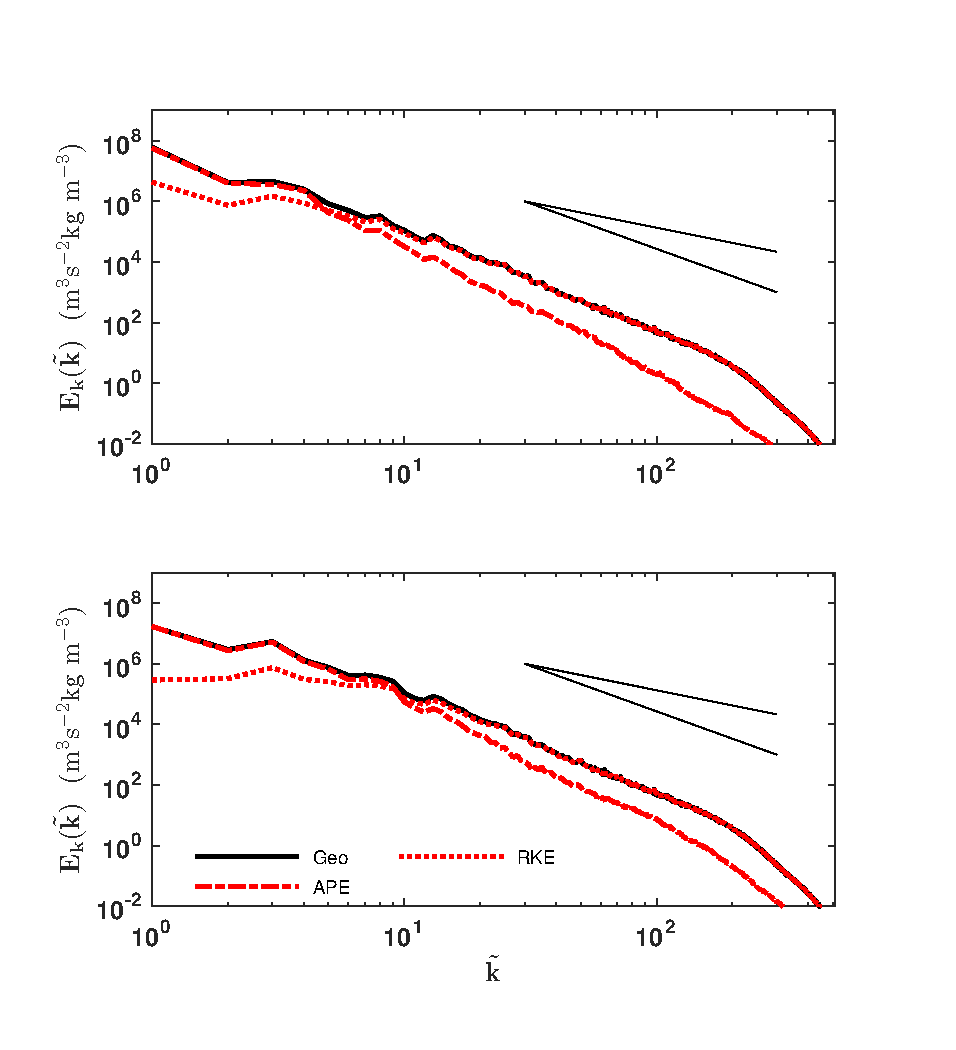
\includegraphics[scale=1]{Chapter4/img/Geo_APERKE_5-7}
\caption{The same as in Figure \ref{fig:Geo_APERKE_1-3}, but for vertical modes 5 (top) and 7 (bottom). The geostrophic mode is mostly overlapped by the RKE. The wavenumber corresponding to $f/c_n$ is $\tilde{k} = 2.5$ for mode 5 and $\tilde{k} = 3.6$ for mode 7.}
\label{fig:Geo_APERKE_5-7}
\end{figure}

\begin{figure}[H]
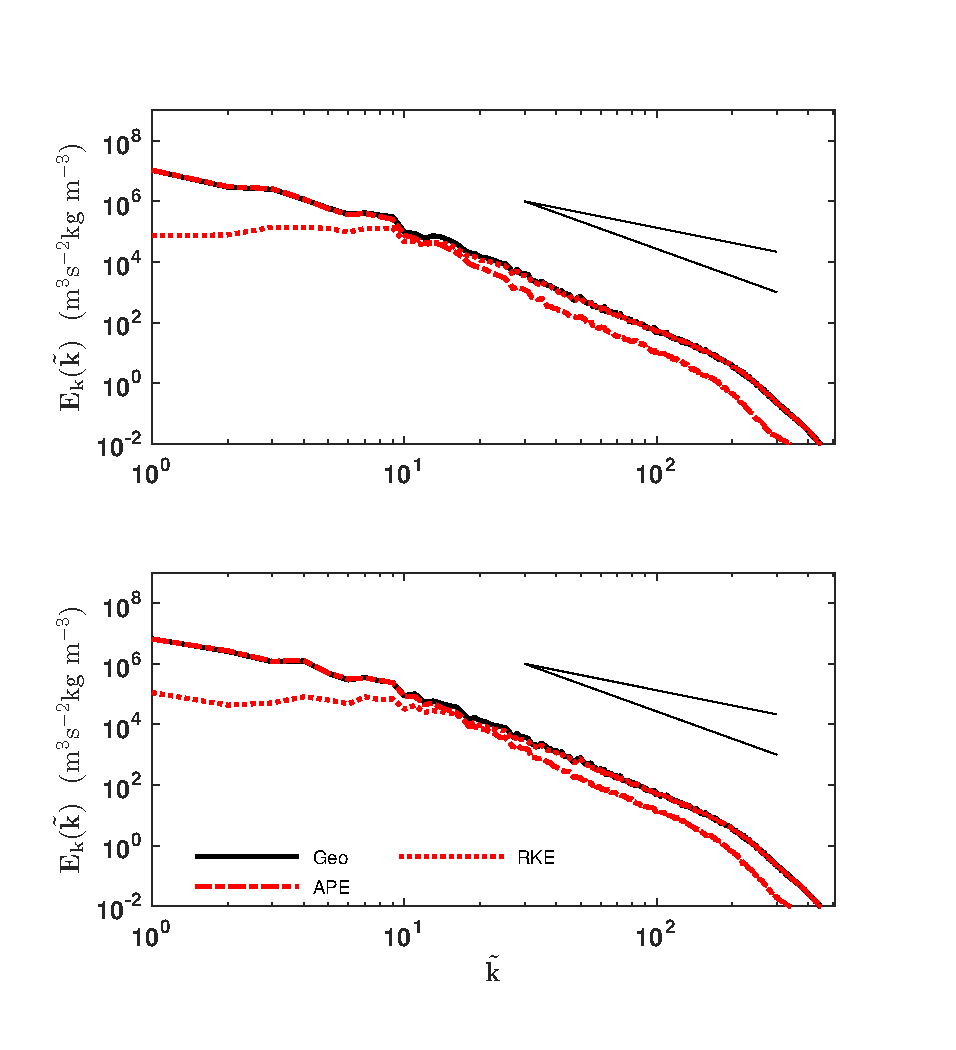
\includegraphics[scale=1]{Chapter4/img/Geo_APERKE_9-11}
\caption{The same as in Figure \ref{fig:Geo_APERKE_1-3}, but for vertical modes 9 (top) and 11 (bottom). The geostrophic mode is mostly overlapped by the APE and RKE. The wavenumber corresponding to $f/c_n$ is $\tilde{k} = 4.9$ for mode 9 and $\tilde{k} = 6.1$ for mode 11.}
\label{fig:Geo_APERKE_9-11}
\end{figure}

\begin{figure}[H]
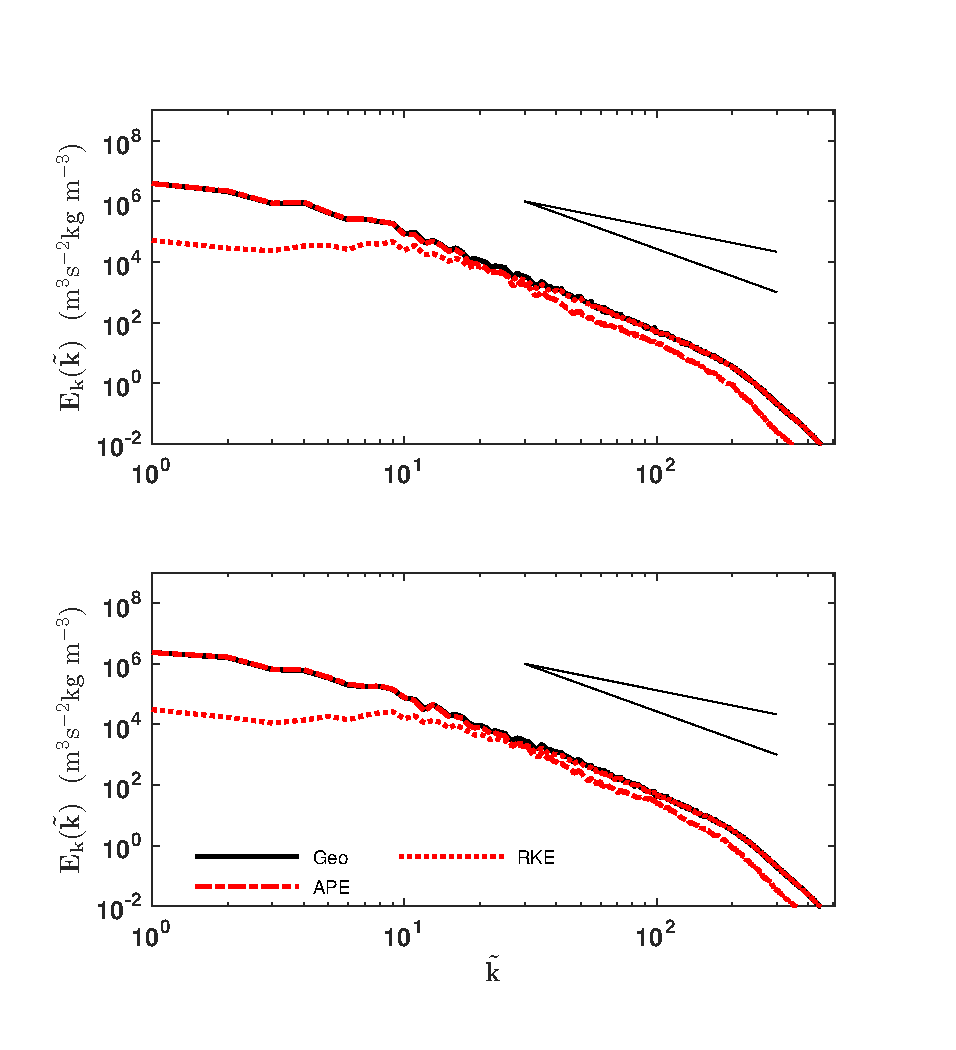
\includegraphics[scale=1]{Chapter4/img/Geo_APERKE_13-15}
\caption{The same as in Figure \ref{fig:Geo_APERKE_1-3}, but for vertical modes 13 (top) and 15 (bottom). The geostrophic mode is mostly overlapped by the APE and RKE. The wavenumber corresponding to $f/c_n$ is $\tilde{k} = 7.5$ for mode 13 and $\tilde{k} = 8.9$ for mode 15.}
\label{fig:Geo_APERKE_13-15}
\end{figure}

\begin{figure}[H]
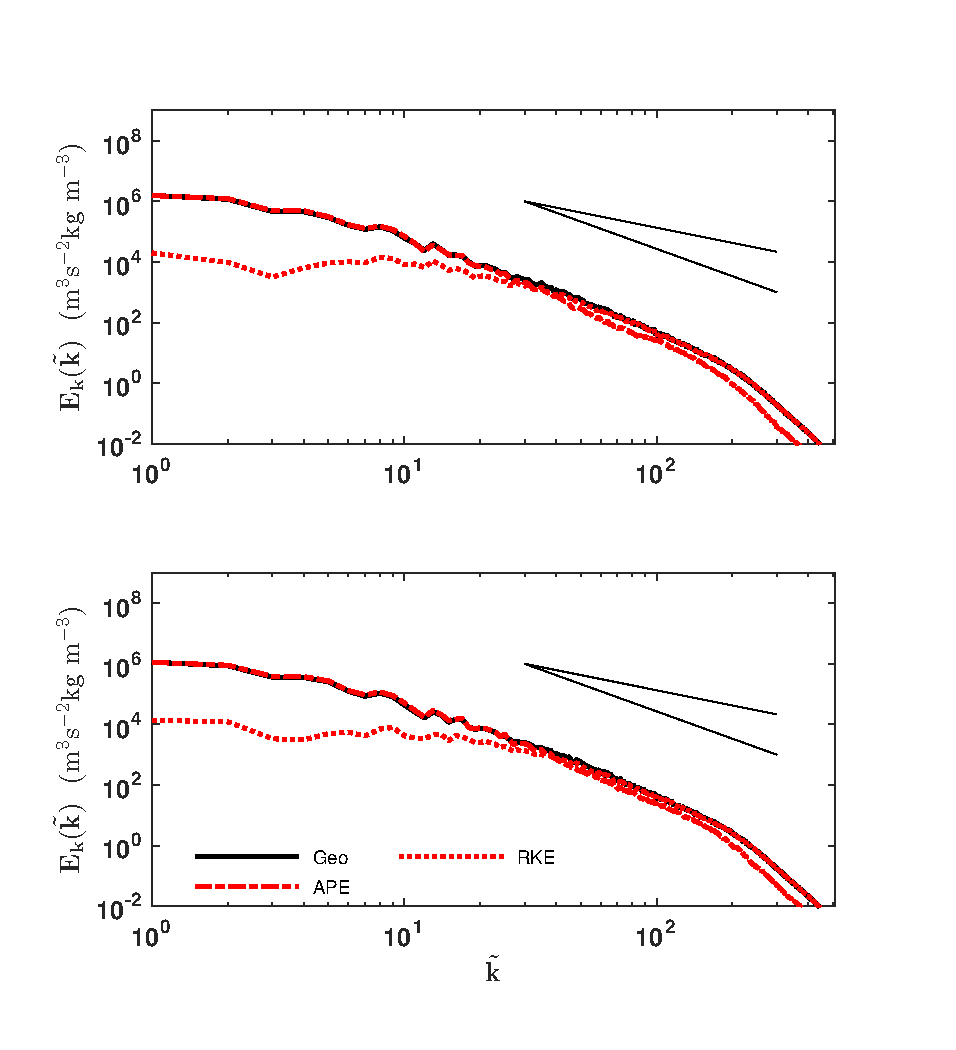
\includegraphics[scale=1]{Chapter4/img/Geo_APERKE_17-19}
\caption{The same as in Figure \ref{fig:Geo_APERKE_1-3}, but for vertical modes 17 (top) and 19 (bottom). The geostrophic mode is mostly overlapped by the APE and RKE. The wavenumber corresponding to $f/c_n$ is $\tilde{k} = 10.3$ for mode 17 and $\tilde{k} = 11.8$ for mode 19.}
\label{fig:Geo_APERKE_17-19}
\end{figure}

\begin{figure}[H]
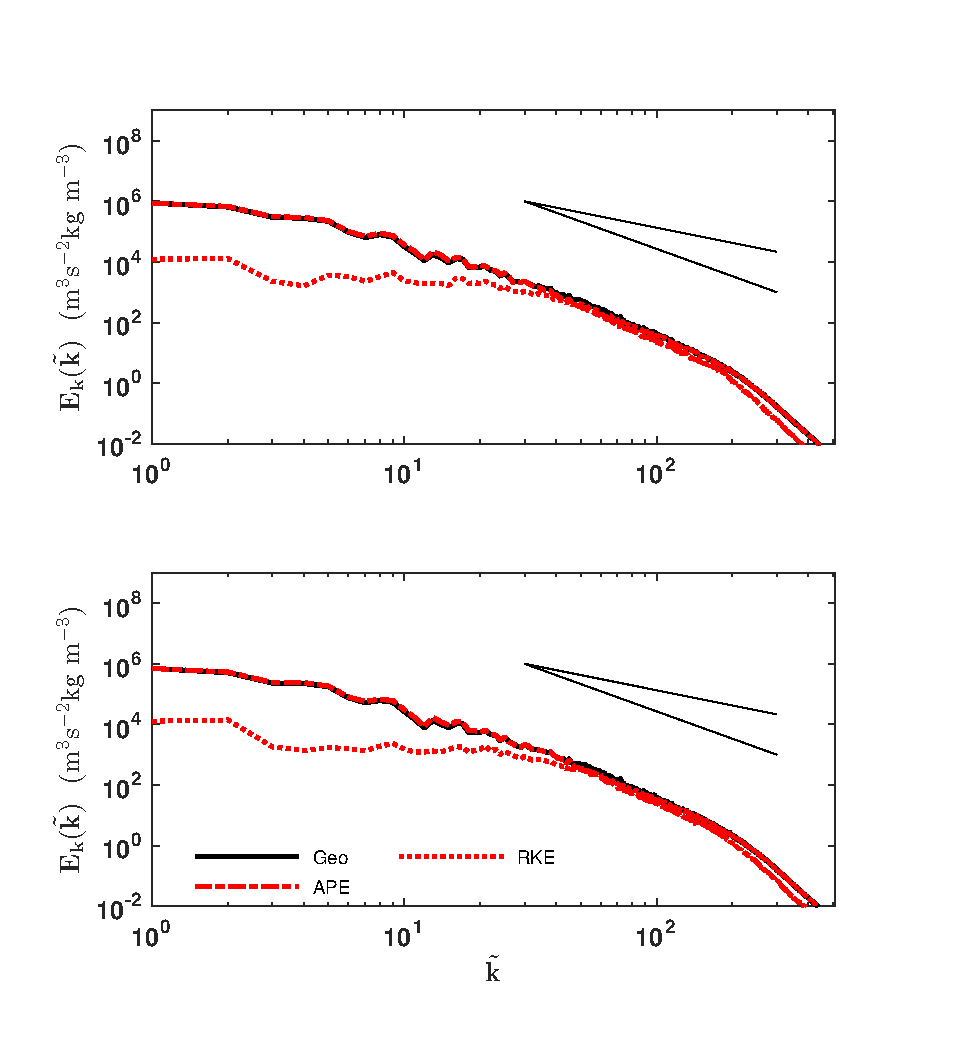
\includegraphics[scale=1]{Chapter4/img/Geo_APERKE_21-23}
\caption{The same as in Figure \ref{fig:Geo_APERKE_1-3}, but for vertical modes 21 (top) and 23 (bottom). The geostrophic mode is mostly overlapped by the APE and RKE. The wavenumber corresponding to $f/c_n$ is $\tilde{k} = 13.4$ for mode 21 and $\tilde{k} = 15$ for mode 23.}
\label{fig:Geo_APERKE_21-23}
\end{figure}

\begin{figure}[H]
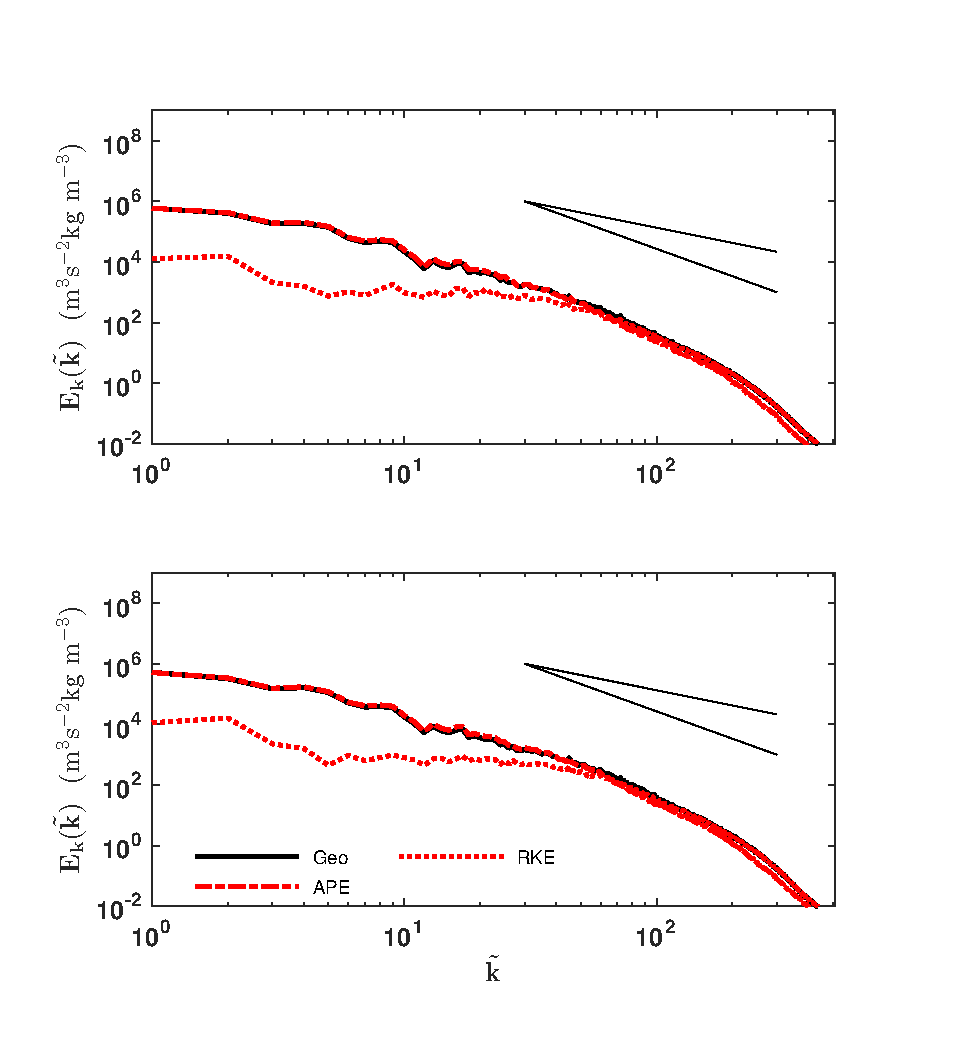
\includegraphics[scale=1]{Chapter4/img/Geo_APERKE_25-27}
\caption{The same as in Figure \ref{fig:Geo_APERKE_1-3}, but for vertical modes 25 (top) and 27 (bottom). The geostrophic mode is mostly overlapped by the APE and RKE. The wavenumber corresponding to $f/c_n$ is $\tilde{k} = 16.6$ for mode 25 and $\tilde{k} = 18.3$ for mode 27.}
\label{fig:Geo_APERKE_25-27}
\end{figure}

\begin{figure}[H]
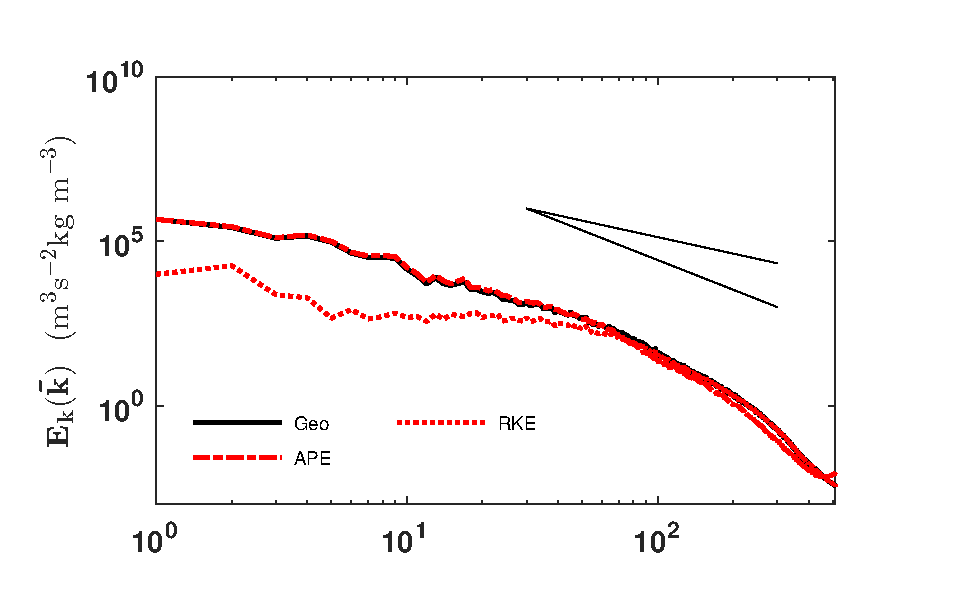
\includegraphics[scale=1]{Chapter4/img/Geo_APERKE_29}
\caption{The same as in Figure \ref{fig:Geo_APERKE_1-3}, but for vertical mode 29. The geostrophic mode is mostly overlapped by the APE and RKE.  The wavenumber corresponding to $f/c_n$ is $\tilde{k} = 20.1$.}
\label{fig:Geo_APERKE_29}
\end{figure}
%%%%%%%%%%%%%%%%%%%%%%%%%%%%%%%%%%%%%%%%%%%%%%%%%%%%%%%%%%%%%%%
\begin{figure}[H]
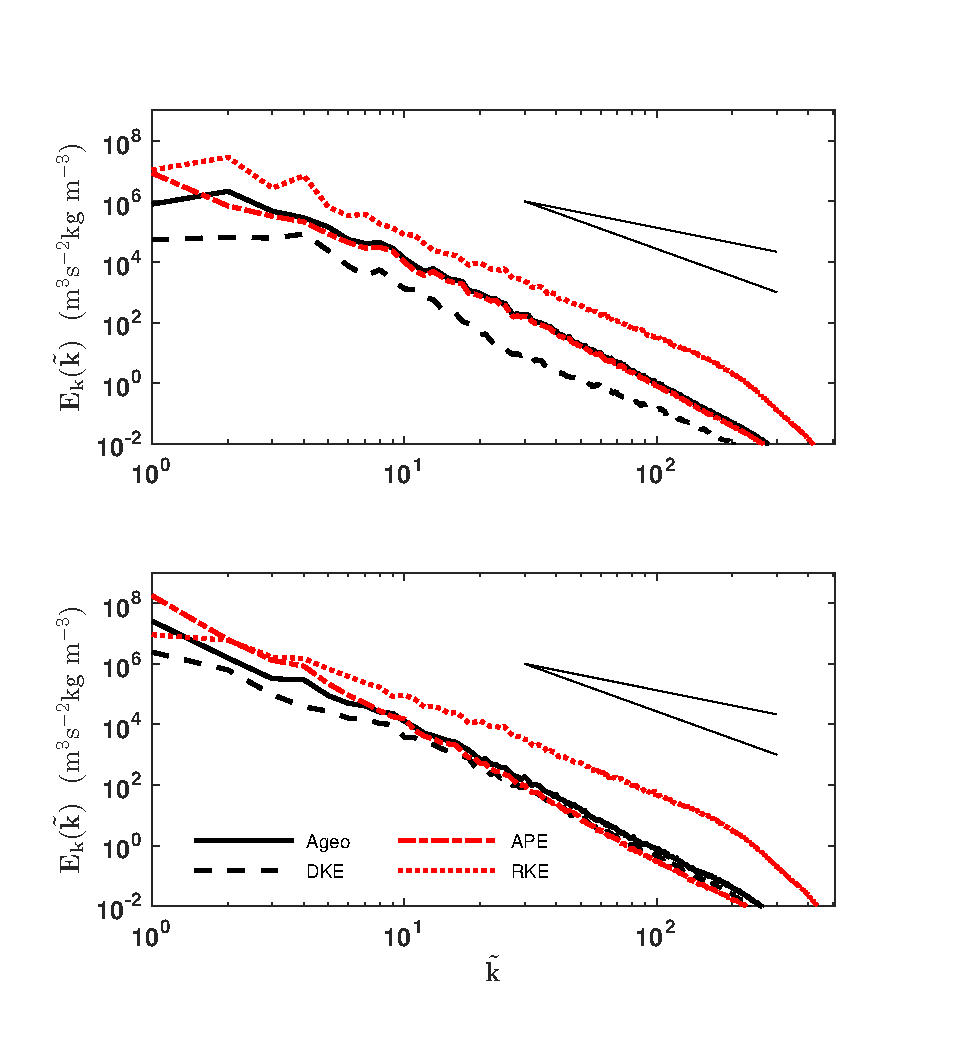
\includegraphics[scale=1]{Chapter4/img/Ageo_APEDKE_1-3}
\caption{Ageostrophic (black solid), DKE (black dashed), APE (red dash-dot), and RKE (red dotted) spectra for vertical modes 1 (top) and 3 (bottom). The wavenumber corresponding to $f/c_n$ is $\tilde{k} = 0.65$ for mode 1 and $\tilde{k} = 1.5$ for mode 3.}
\label{fig:Ageo_APEDKE_1-3}
\end{figure}

\begin{figure}[H]
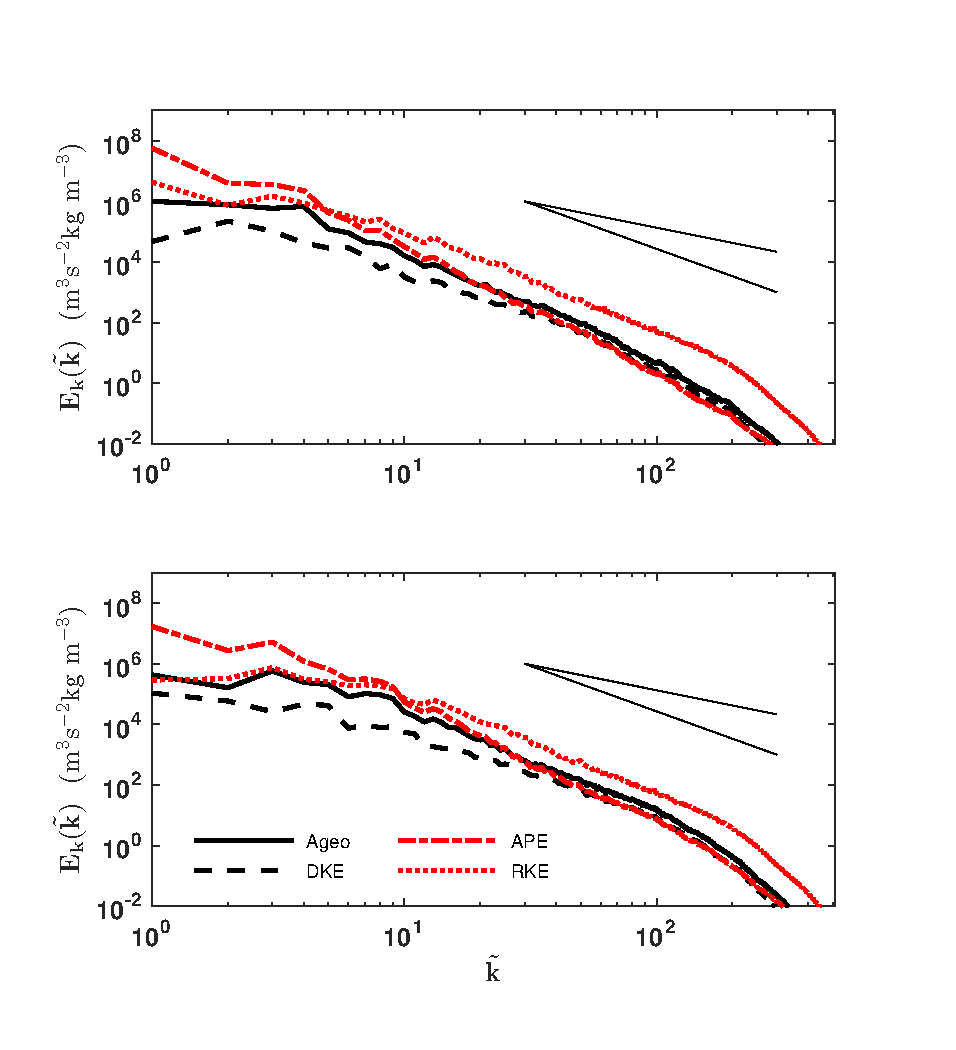
\includegraphics[scale=1]{Chapter4/img/Ageo_APEDKE_5-7}
\caption{The same as in Figure \ref{fig:Ageo_APEDKE_1-3}, but for vertical modes 5 (top) and 7 (bottom). The wavenumber corresponding to $f/c_n$ is  $\tilde{k} = 2.5$ for mode 5 and $\tilde{k} = 3.6$ for mode 7.}
\label{fig:Ageo_APEDKE_5-7}
\end{figure}

\begin{figure}[H]
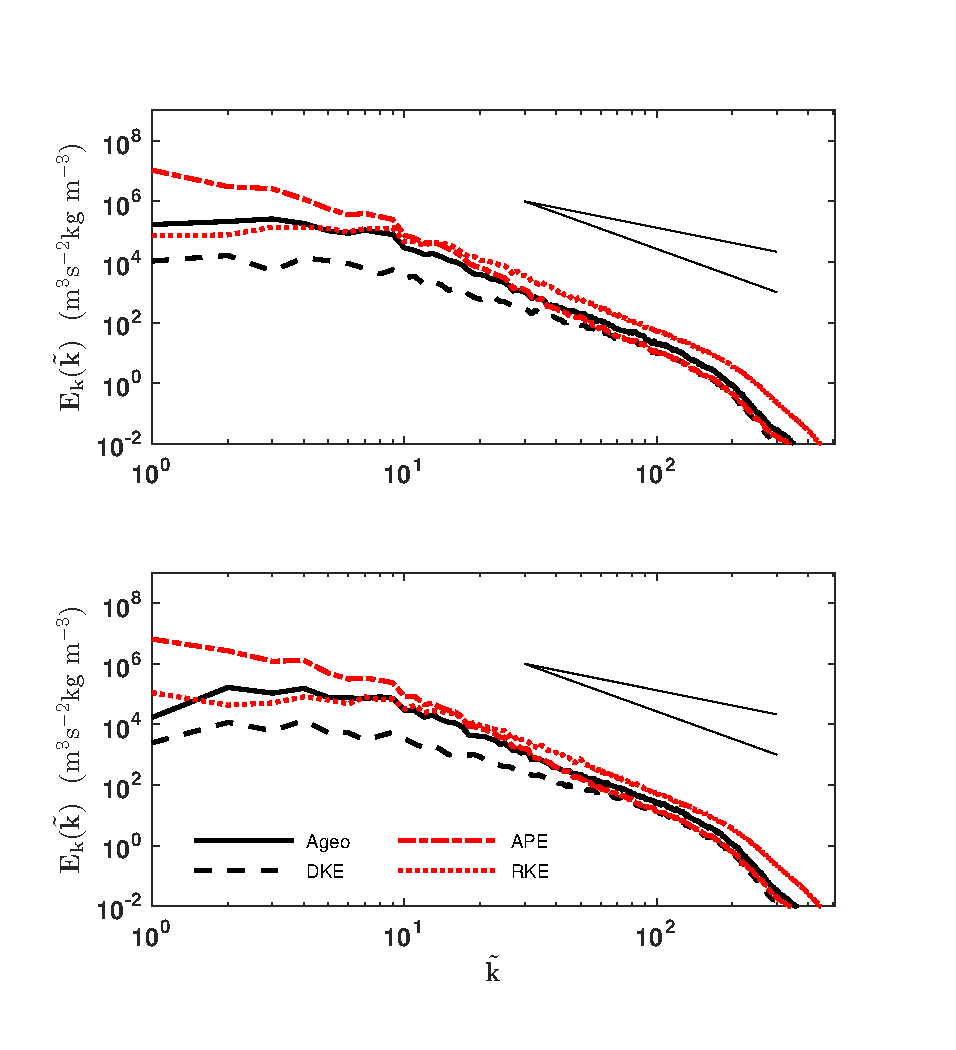
\includegraphics[scale=1]{Chapter4/img/Ageo_APEDKE_9-11}
\caption{The same as in Figure \ref{fig:Ageo_APEDKE_1-3}, but for vertical modes 9 (top) and 11 (bottom).  The wavenumber corresponding to $f/c_n$ is $\tilde{k} = 4.9$ for mode 9 and $\tilde{k} = 6.1$ for mode 11.}
\label{fig:Ageo_APEDKE_9-11}
\end{figure}

\begin{figure}[H]
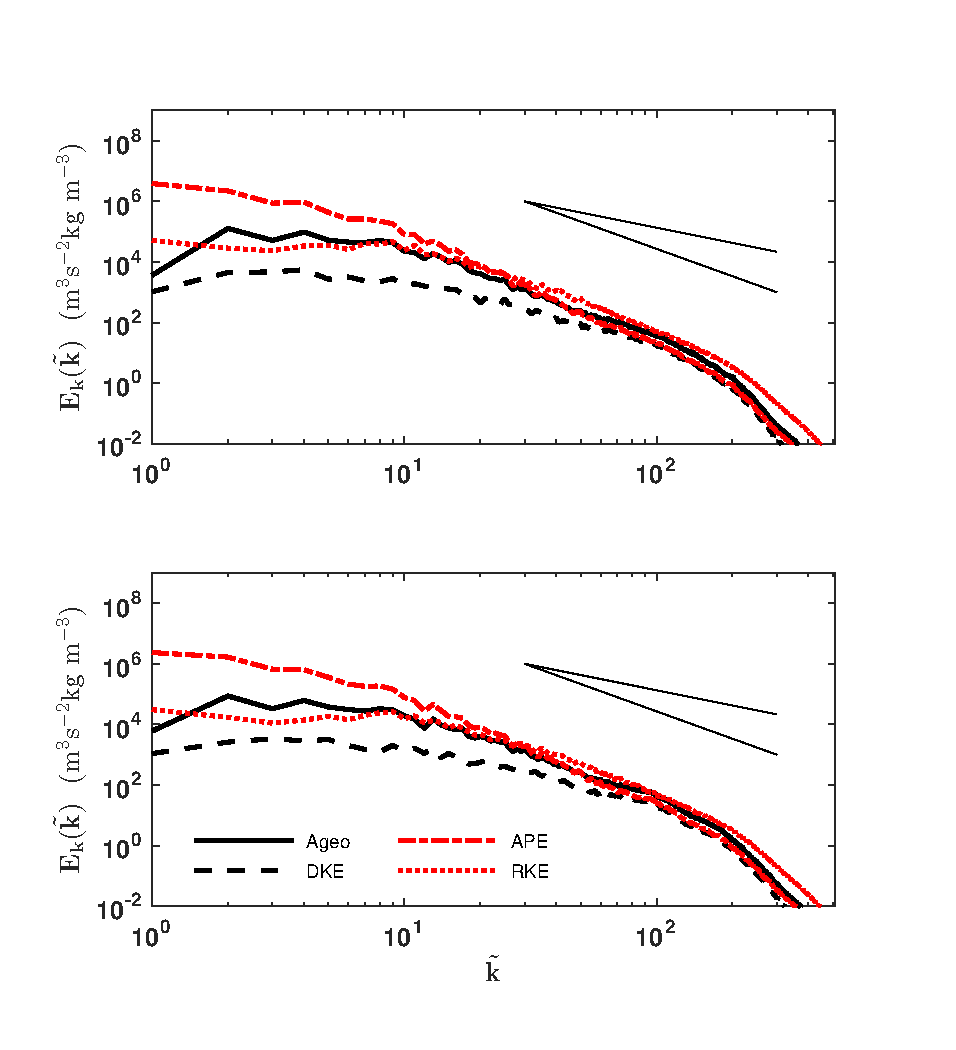
\includegraphics[scale=1]{Chapter4/img/Ageo_APEDKE_13-15}
\caption{The same as in Figure \ref{fig:Ageo_APEDKE_1-3}, but for vertical modes 13 (top) and 15 (bottom). The wavenumber corresponding to $f/c_n$ is $\tilde{k} = 7.5$ for mode 13 and $\tilde{k} = 8.9$ for mode 15.}
\label{fig:Ageo_APEDKE_13-15}
\end{figure}

\begin{figure}[H]
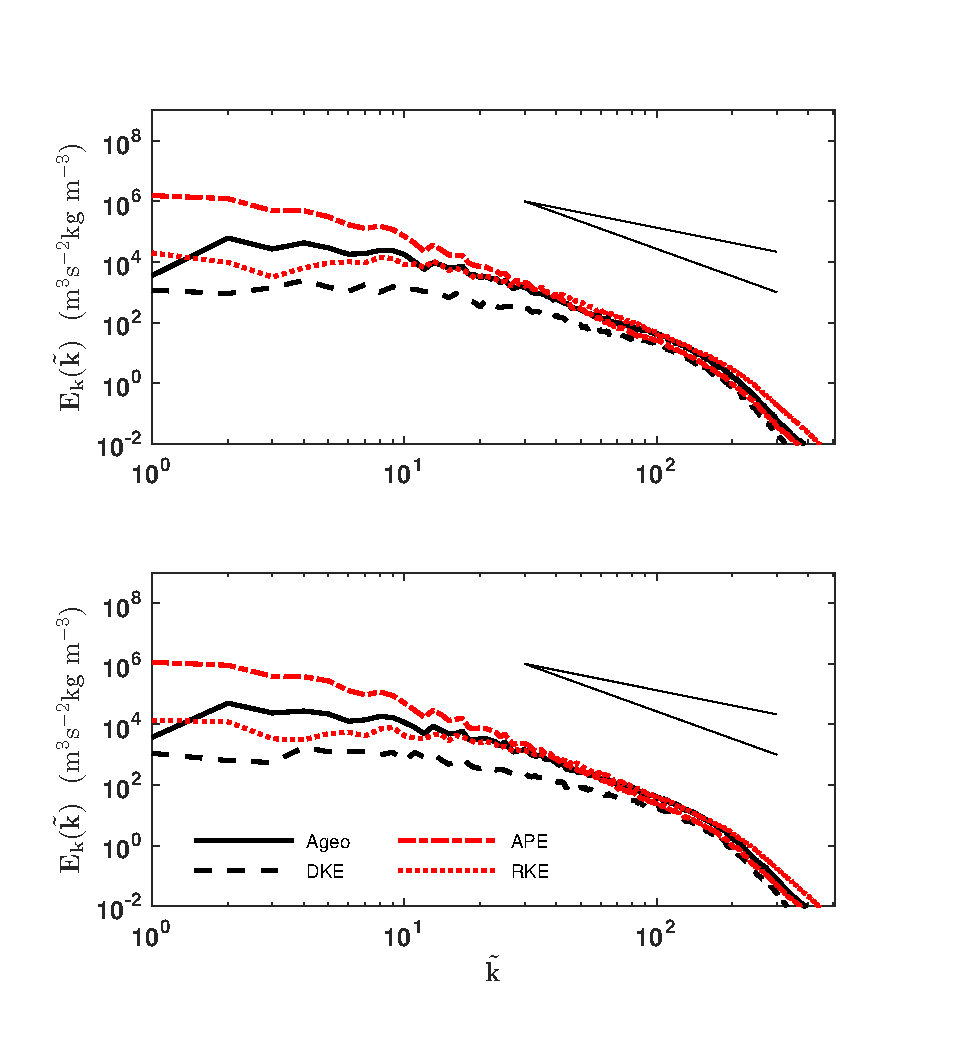
\includegraphics[scale=1]{Chapter4/img/Ageo_APEDKE_17-19}
\caption{The same as in Figure \ref{fig:Ageo_APEDKE_1-3}, but for vertical modes 17 (top) and 19 (bottom). The wavenumber corresponding to $f/c_n$ is $\tilde{k} = 10.3$ for mode 17 and $\tilde{k} = 11.8$ for mode 19.}
\label{fig:Ageo_APEDKE_17-19}
\end{figure}

\begin{figure}[H]
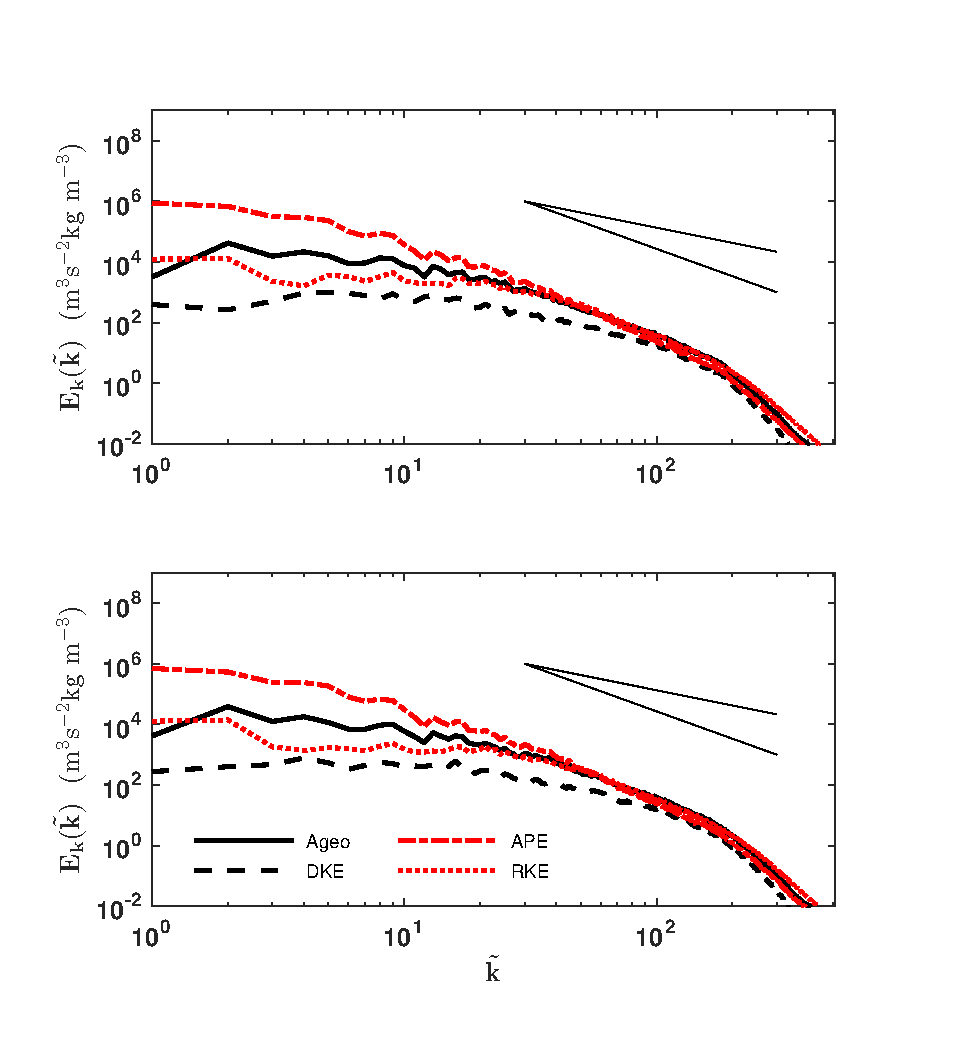
\includegraphics[scale=1]{Chapter4/img/Ageo_APEDKE_21-23}
\caption{The same as in Figure \ref{fig:Ageo_APEDKE_1-3}, but for vertical modes 21 (top) and 23 (bottom). The wavenumber corresponding to $f/c_n$ is $\tilde{k} = 13.4$ for mode 21 and $\tilde{k} = 15$ for mode 23.}
\label{fig:Ageo_APEDKE_21-23}
\end{figure}

\begin{figure}[H]
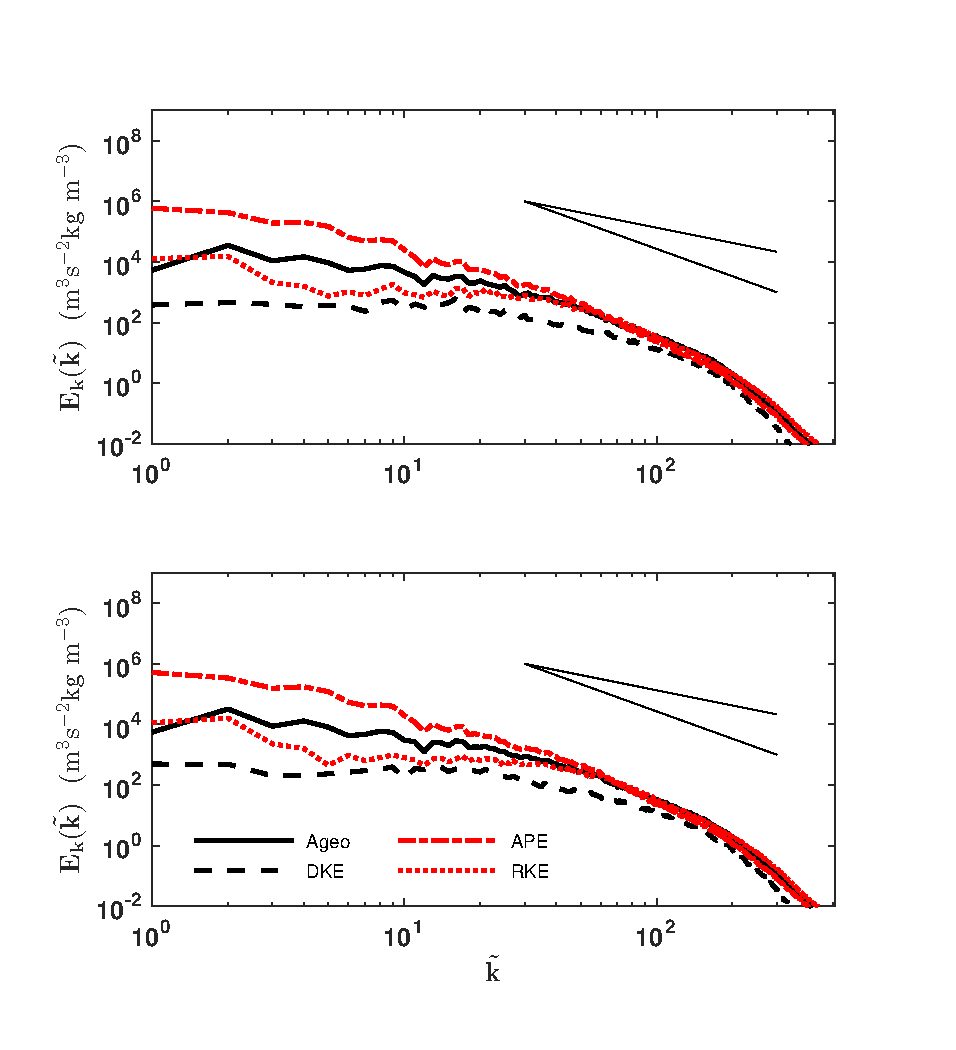
\includegraphics[scale=1]{Chapter4/img/Ageo_APEDKE_25-27}
\caption{The same as in Figure \ref{fig:Ageo_APEDKE_1-3}, but for vertical modes 25 (top) and 27 (bottom). The wavenumber corresponding to $f/c_n$ is $\tilde{k} = 16.6$ for mode 25 and $\tilde{k} = 18.3$ for mode 27.}
\label{fig:Ageo_APEDKE_25-27}
\end{figure}

\begin{figure}[H]
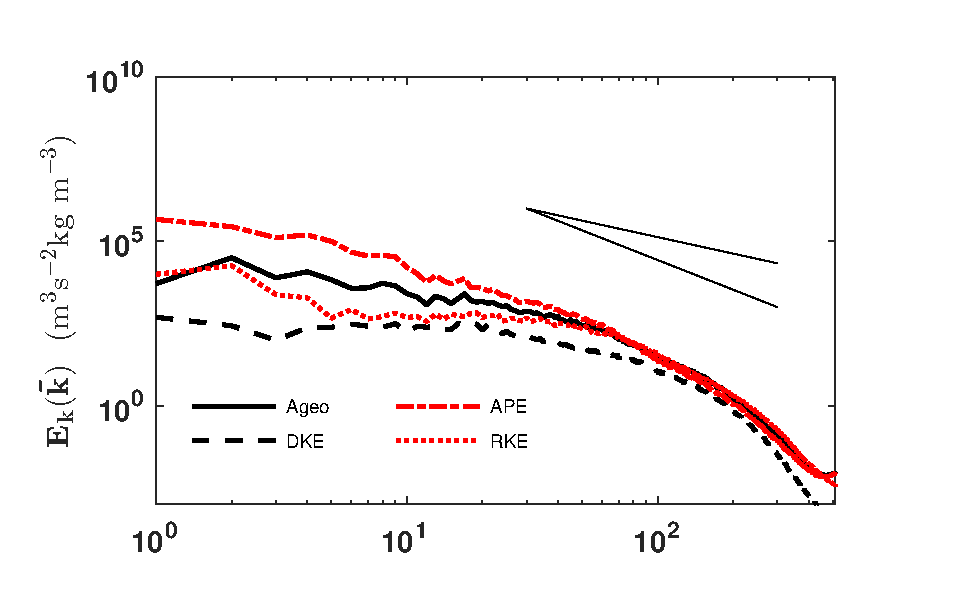
\includegraphics[scale=1]{Chapter4/img/Ageo_APEDKE_29}
\caption{The same as in Figure \ref{fig:Ageo_APEDKE_1-3}, but for vertical mode 29. The wavenumber corresponding to $f/c_n$ for this mode is $\tilde{k} = 20.1$.}
\label{fig:Ageo_APEDKE_29}
\end{figure}

In addition to examining the spectra of the individual vertical modes, it could be more enlightening to study the mesoscale slopes of the geostrophic, ageostrophic, and Helhmoltz modes as a function of vertical mode number. Table \ref{tab:slopes} shows the slope of the geostrophic, ageostrophic, RKE, and DKE in the mesoscale, calculated over the interval $6 \leq \tilde{k} \leq 60$. $R^2 > 0.94$ for every mode. Clearly, the general trend is that the slopes of all of the spectra decrease as the vertical mode number increases.  In addition to Table \ref{tab:slopes}, this can be more easily seen in the accompanying Figure \ref{fig:slopes}.\\

Overall, geostrophic mesoscale slopes are around -3 or steeper for vertical modes $<$ 15. The ageostrophic mesoscale spectrum shallows for vertical modes $>$ 10. The RKE and DKE spectra are much shallower than the geostrophic and ageostrophic spectra for largest values of $n$.

\begin{table}[H]
\begin{tabular}{c c c c c}
\hline
\textbf{Vertical Mode} & \textbf{Geostrophic Slope} & \textbf{RKE slope} & \textbf{Ageostrophic Slope} & \textbf{DKE slope}\\
\hline
Barotropic (0) & -3.6 & -3.6 & -4.0 & -3.1 \\
1 & -3.4 & -3.4 & -4.0 & -4.3\\
2 & -3.2 & -3.2 & -4.6 & -4.8\\
3 & -3.2 & -3.2 & -4.1 & -4.0\\
4 & -3.3 & -3.2 & -3.6 & -3.3\\
5 & -3.4 & -3.3 & -3.2 & -2.8\\
6 & -3.4 & -3.2 & -3.3 & -2.7\\
7 & -3.5 & -3.2 & -3.4 & -2.6 \\
8 & -3.5 & -3.1 & -3.4 & -2.5 \\
9 & -3.4 & -3.0 & -3.3 & -2.3 \\
10 & -3.4 & -2.8 & -3.2 & -2.2 \\
11 & -3.3 & -2.7 & -3.2 & -2.2 \\
12 & -3.2 & -2.6 & -3.0 & -2.1\\
13 & -3.2 & -2.4 & -2.9 & -2.0 \\
14 & -3.1 & -2.2 & -2.8 & -1.9\\
15 & -3.0 & -2.1 & -2.7 & -1.8\\
16 & -2.9 & -2.0 & -2.5 & -1.7\\
17 & -2.9 & -1.9 & -2.4 & -1.6\\
18 & -2.8 & -1.7 & -2.3 & -1.5\\
19 & -2.7 & -1.5 & -2.2 & -1.5\\
20 & -2.7 & -1.4 & -2.1 & -1.4\\
21 & -2.6 & -1.3 & -2.0 & -1.3\\
22 & -2.5 & -1.1 & -2.0 & -1.3\\
23 & -2.5 & -1.0 & -1.9 & -1.2\\
24 & -2.4 & -0.93 & -1.8 & -1.2\\
25 & -2.3 & -0.82 & -1.7 & -1.2\\
26 & -2.3 & -0.73 & -1.6 & -1.1\\
27 & -2.2 & -0.67 & -1.5 & -1.1\\
28 & -2.2 & -0.63 & -1.5 & -1.0\\
29 & -2.2 & -0.57 & -1.4 & -1.0 \\
30 & -2.1 & -0.56 & -1.4 & -0.96\\
\hline
\end{tabular}
\caption{The spectra slopes of the first 30 modes in the mesoscale.}
\label{tab:slopes}
\end{table}

\begin{figure}[H]
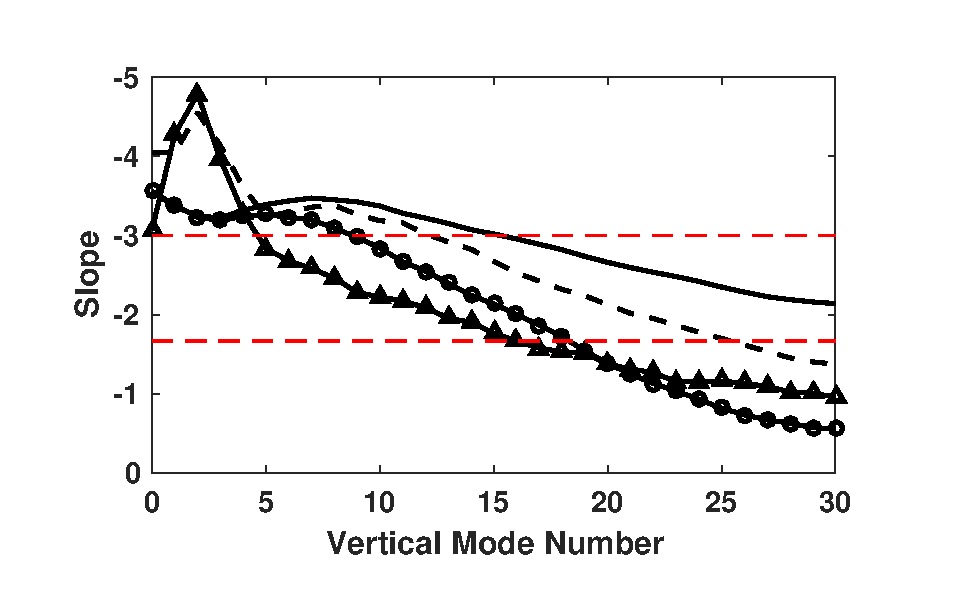
\includegraphics[scale=1]{Chapter4/img/slopes}
\caption{The mesoscale spectra slopes of the geostrophic (solid), ageostrophic (dashed), RKE (circles), and DKE (triangles) as a function of vertical mode number. Red dashed lines show references to $-3$ and $-5/3$ slopes. Note that the y-axis is reversed so that more negative values (i.e. steeper slope values) appear higher on the y-axis.}
\label{fig:slopes}
\end{figure}

Lastly, to determine the relative importance of each vertical mode in the full decomposition of the baroclinic jet into balanced vortical and inertia-gravity wave motion, the fraction of energy in each vertical mode is shown in Figure \ref{fig:modal_energy}. A large fraction of the energy is in the barotropic mode, so to help illustrate the contributions of the baroclinic modes, Figure \ref{fig:modal_energy_nobaro} shows the energy distribution, excluding the barotropic mode.\\

Since the mesoscale spectra are of particular interest, we also calculate the fraction of energy of each vertical mode contained in the mesoscale. This mesoscale energy is decomposed into geostrophic and ageostrophic components and displayed in Figure \ref{fig:meso_GeoAgeo}. The KE and APE in each vertical mode in shown as well in Figure \ref{fig:meso_KEPE}.

\begin{figure}[H]
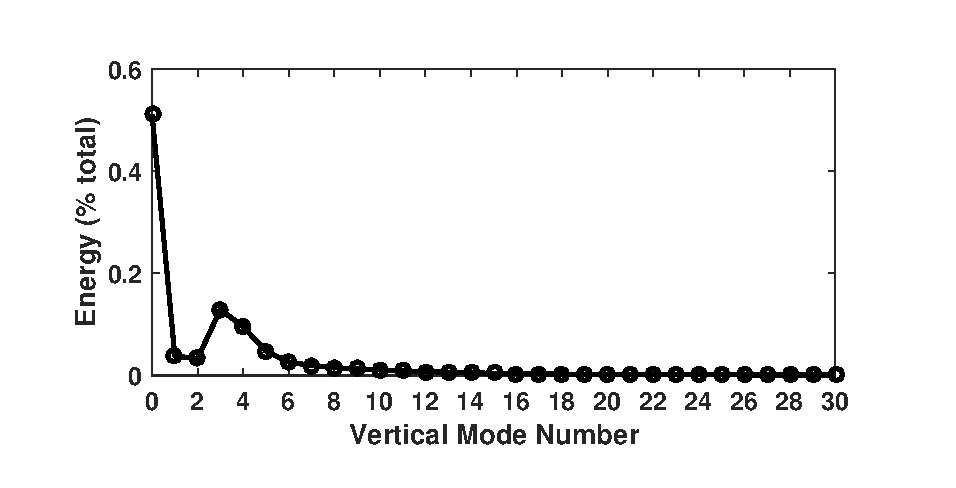
\includegraphics[scale=1]{Chapter4/img/modal_energy}
\caption{The fraction of energy in each vertical mode.}
\label{fig:modal_energy}
\end{figure}
\vspace{-0.2in}
\begin{figure}[H]
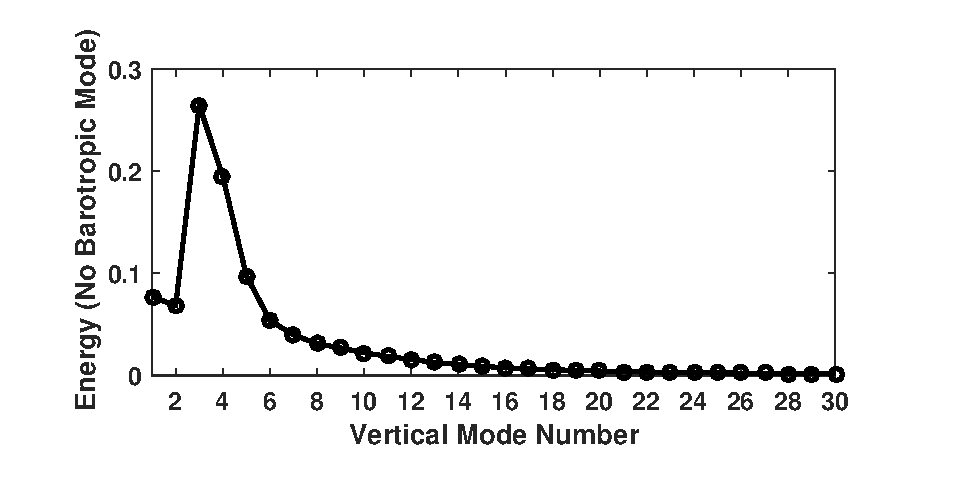
\includegraphics[scale=1]{Chapter4/img/modal_energy_nobaro}
\caption{As in Figure \ref{fig:meso_GeoAgeo},  excluding the barotropic mode.}
\label{fig:modal_energy_nobaro}
\end{figure}

\begin{figure}[H]
\vspace{0cm}
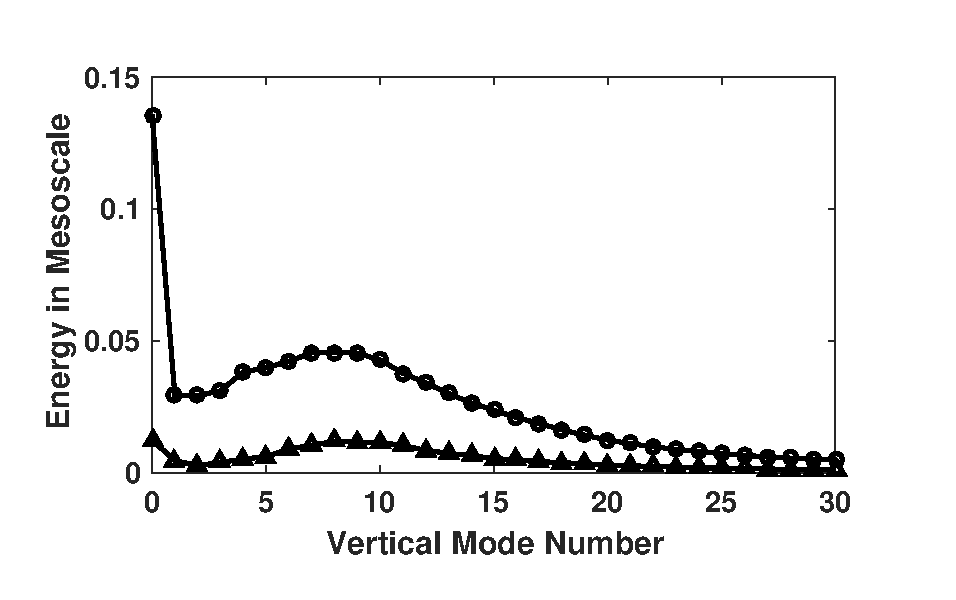
\includegraphics[scale=1]{Chapter4/img/meso_GeoAgeo}
\vspace{0cm}
\caption{The fraction of mesoscale energy in each vertical mode for the geostrophic (circles) and ageostrophic (triangles) modes.}
\label{fig:meso_GeoAgeo}
\end{figure}

\begin{figure}[H]
\vspace{0cm}
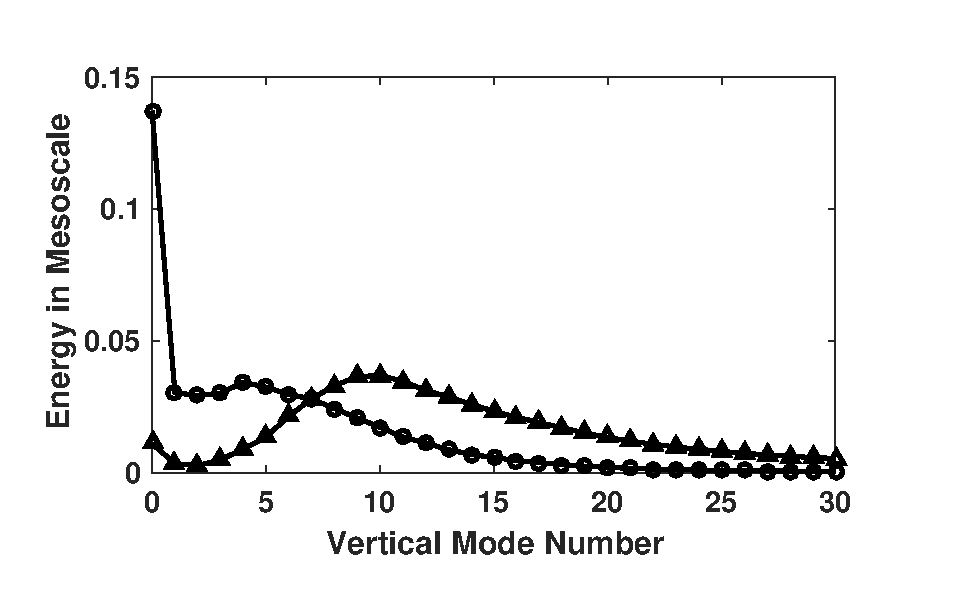
\includegraphics[scale=1]{Chapter4/img/meso_KEPE}
\vspace{0cm}
\caption{As in Figure \ref{fig:meso_GeoAgeo}, but for the KE (circles) and APE (triangles).}
\label{fig:meso_KEPE}
\end{figure}

\subsection{Combining the Vertical Modes}
Due to the orthogonality of the normal mode decomposition, by summing the first 30 vertical modes the normal mode decomposition can be compared to the depth-averaged Helmholtz decomposition of the full velocity fields (see Figure \ref{fig:totalGeoAgeo}).  As seen, the geostrophic and RKE slopes are -3.1 and -2.7, respectively. There is a bit more discrepancy between the ageostrophic and DKE slopes with values of -2.7 and -1.9, respectively. 

\begin{figure}[H]
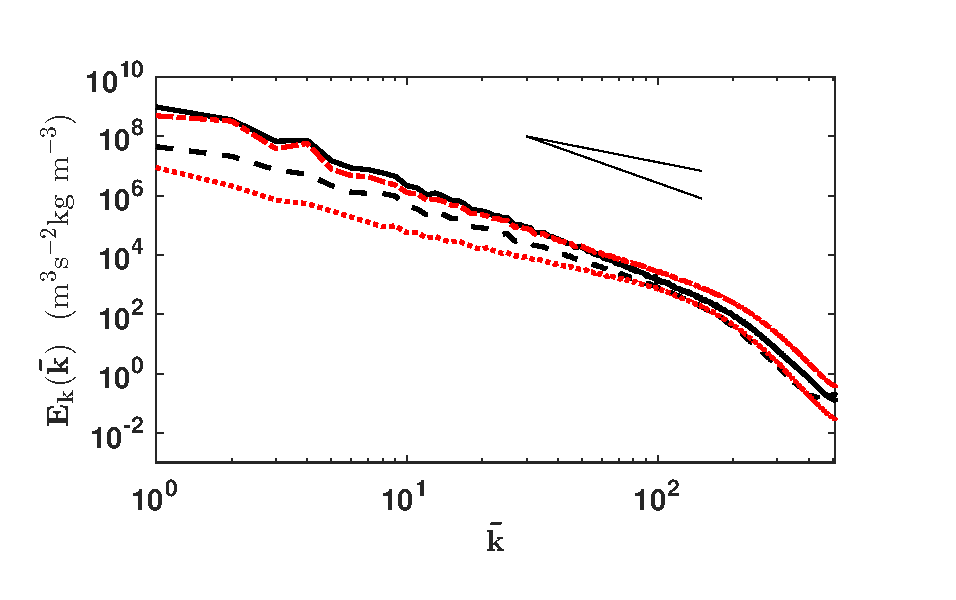
\includegraphics[scale=1]{Chapter4/img/totalGeoAgeo}
\vspace{-0.5in}
\caption{The first 30 vertical modes summed together (geostrophic, black solid; ageostrophic, black dashed) compared to the vertically-averaged RKE (red dash-dot) and DKE (red dotted). $-3$ and $-5/3$ references are shown in the upper right.}
\label{fig:totalGeoAgeo}
\end{figure}

From  Figure \ref{fig:meso_GeoAgeo}, it appears that (excluding the barotropic mode), a lot of the mesoscale energy lies between vertical modes 5 and 15. To investigate this,  Figure \ref{fig:meso_RKEDKE} shows the normal mode decomposition and Helmholtz decomposition summed over vertical modes 5 through 15. The geostrophic and ageostrophic slopes are -3.3 and -3.1, while the RKE and DKE slopes are -2.9 and -2.3.\\

\begin{figure}[H]
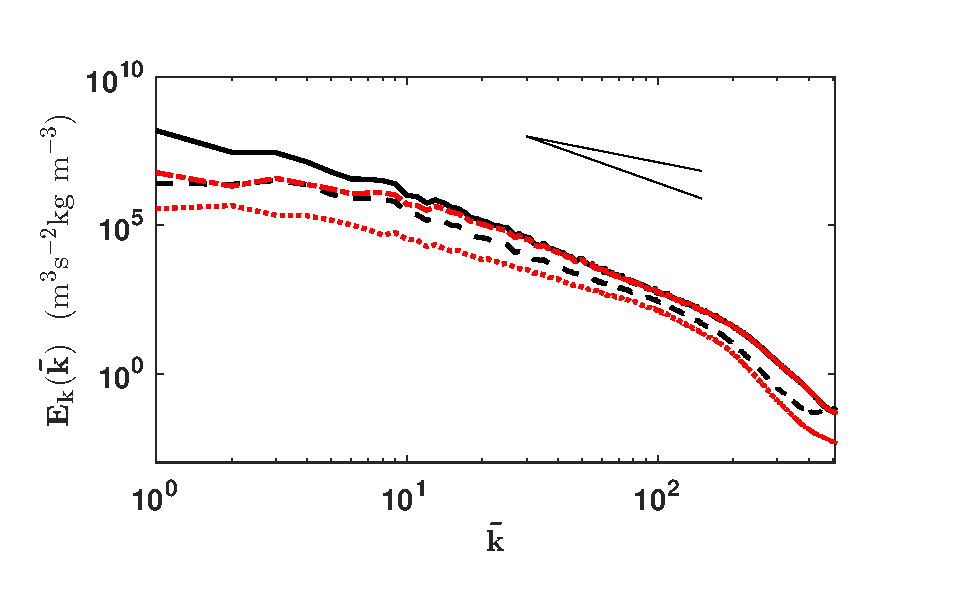
\includegraphics[scale=1]{Chapter4/img/meso_RKEDKE}
\caption{The geostrophic (black solid) and ageostrophic (black dashed) compared to the RKE (red dash-dot) and DKE (red dotted) spectra summed over vertical modes 5 through 15. $-3$ and $-5/3$ references are shown in the upper right.}
\label{fig:meso_RKEDKE}
\end{figure}

In Chapter \ref{ch:ch5}, we discuss these results and offer an explanation for the mesoscale spectra of the full decomposition as seen in Figure \ref{fig:totalGeoAgeo}.